%% abtex2-modelo-trabalho-academico.tex, v-1.9.6 laurocesar
%% Copyright 2012-2016 by abnTeX2 group at http://www.abntex.net.br/ 
%%
%% This work may be distributed and/or modified under the
%% conditions of the LaTeX Project Public License, either version 1.3
%% of this license or (at your option) any later version.
%% The latest version of this license is in
%%   http://www.latex-project.org/lppl.txt
%% and version 1.3 or later is part of all distributions of LaTeX
%% version 2005/12/01 or later.
%%
%% This work has the LPPL maintenance status `maintained'.
%% 
%% The Current Maintainer of this work is the abnTeX2 team, led
%% by Lauro César Araujo. Further information are available on 
%% http://www.abntex.net.br/
%%
%% This work consists of the files abntex2-modelo-trabalho-academico.tex,
%% abntex2-modelo-include-comandos and abntex2-modelo-references.bib
%%

% ------------------------------------------------------------------------
% ------------------------------------------------------------------------
% abnTeX2: Modelo de Trabalho Academico (tese de doutorado, dissertacao de
% mestrado e trabalhos monograficos em geral) em conformidade com 
% ABNT NBR 14724:2011: Informacao e documentacao - Trabalhos academicos -
% Apresentacao
% ------------------------------------------------------------------------
% ------------------------------------------------------------------------

% Link for source code:
% https://github.com/abntex/abntex2/blob/master/doc/latex/abntex2/examples/abntex2-modelo-trabalho-academico.tex

% abntex2cite reference:
% http://mirrors.ibiblio.org/CTAN/macros/latex/contrib/abntex2/doc/abntex2cite.pdf
% http://mirrors.ibiblio.org/CTAN/macros/latex/contrib/abntex2/doc/abntex2cite-alf.pdf

\documentclass[
	% -- opções da classe memoir --
	12pt,				% tamanho da fonte
	openright,			% capítulos começam em pág ímpar (insere página vazia caso preciso)
	a4paper,			% tamanho do papel. 
	oneside,
	% -- opções da classe abntex2 --
	%chapter=TITLE,		% títulos de capítulos convertidos em letras maiúsculas
	%section=TITLE,		% títulos de seções convertidos em letras maiúsculas
	%subsection=TITLE,	% títulos de subseções convertidos em letras maiúsculas
	%subsubsection=TITLE,% títulos de subsubseções convertidos em letras maiúsculas
	% -- opções do pacote babel --
    %brazil		        % idioma adicional para hifenização
	%french,		    % idioma adicional para hifenização
	%spanish,			% idioma adicional para hifenização
	english,		    % o último idioma é o principal do documento
	hyphens
]{abntex2}

% ---
% Pacotes básicos 
% ---
\usepackage{lmodern}			% Usa a fonte Latin Modern			
\usepackage[T1]{fontenc}		% Selecao de codigos de fonte.
\usepackage[utf8]{inputenc}		
\usepackage{lastpage}			% Usado pela Ficha catalográfica
\usepackage{indentfirst}		% Indenta o primeiro parágrafo de cada seção.
\usepackage{color}				% Controle das cores
\usepackage{graphicx}			% Inclusão de gráficos
\usepackage{microtype} 			% para melhorias de justificação
\usepackage{multirow}
\usepackage{multicol}
\usepackage{mathptmx}
\usepackage{xspace}
\usepackage{pdfpages}
\usepackage{float}
\usepackage{booktabs}
\usepackage[ruled,vlined]{algorithm2e}
%\usepackage[style=abnt]{biblatex}

% Pacotes de citações
\usepackage[english,hyperpageref]{backref}	 % Paginas com as citações na bibl
\usepackage[alf]{abntex2cite}	% Citações padrão ABNT
%\addbibresource{reference.bib}
% ---

\renewcommand{\arraystretch}{1.3}

% --- 
% CONFIGURAÇÕES DE PACOTES
% --- 

% ---
% Configurações do pacote backref
% Usado sem a opção hyperpageref de backref
\renewcommand{\backrefpagesname}{Cited in page(s):~}
\renewcommand{\backref}{}
\renewcommand*{\backrefalt}[4]{
	\ifcase #1 %
		No citation in text.%
	\or
		Cited in page #2.%
	\else
		Cited #1 times in pages #2.%
	\fi}%

% ---
% \newcommand{\ava}{ambiente virtual de aprendizagem\xspace}

% ---
% Informações de dados para CAPA e FOLHA DE ROSTO
% ---
\titulo{Representation of the Computer Vision of Autonomous Vehicles using Computer Graphics}
\autor{\large Felipe Marinho Tavares\\ João Guilherme de Souza Alves Costa}
\local{Itabira}
\data{2018}
\orientador{Giovani Bernardes Vitor}
\instituicao{%
  Universidade Federal de Itajubá -- UNIFEI
  \par
  Computer Engineering
  \par
  Itabira Campus}
\tipotrabalho{Undergraduate Thesis}
% O preambulo deve conter o tipo do trabalho, o objetivo, 
% o nome da instituição e a área de concentração 
\preambulo{Undergraduate Thesis presented to the Universidade Federal de Itajubá - Itabira Campus as a requirement for the conclusion of the Computer Engineering undergraduate degree under the guidance of Dr. Giovani Bernardes Vitor.}
% ---

% ---
% Configurações de aparência do PDF final

% alterando o aspecto da cor azul
\definecolor{blue}{RGB}{41,5,195}

% informações do PDF
\makeatletter
\hypersetup{
     	%pagebackref=true,
		pdftitle={\@title},
		pdfauthor={\@author},
    	pdfsubject={\imprimirpreambulo},
	    pdfcreator={LaTeX with abnTeX2},
		pdfkeywords={abnt}{latex}{abntex}{abntex2}{trabalho acadêmico}, 
		colorlinks=true,       		% false: boxed links; true: colored links
    	linkcolor=black,          	% color of internal links
    	citecolor=black,        	% color of links to bibliography
    	filecolor=magenta,      	% color of file links
		urlcolor=black,
		bookmarksdepth=4
}
\makeatother
% --- 

% --- 
% Espaçamentos entre linhas e parágrafos 
% --- 

% O tamanho do parágrafo ao dado por:
\setlength{\parindent}{1.3cm}

% Controle do espaçamento entre um parágrafo e outro:
\setlength{\parskip}{0.2cm}  % tente também \onelineskip

% ---
% compila o indice
% ---
\makeindex
% ---

% ----
% Início do documento
% ----
\begin{document}

% Seleciona o idioma do documento (conforme pacotes do babel)
\selectlanguage{english}

% Retira espaço extra obsoleto entre as frases.
\frenchspacing 

% ----------------------------------------------------------
% ELEMENTOS PRÉ-TEXTUAIS
% ----------------------------------------------------------
% \pretextual

% ---
% Capa
% ---
\imprimircapa
% ---

% ---
% Folha de rosto
% (o * indica que haverá¡ a ficha bibliográfica)
% ---
\imprimirfolhaderosto*
% ---

% ---
% Inserir a ficha bibliografica
% ---

%% Isto é um exemplo de Ficha Catalográfica, ou ``Dados internacionais de
% catalogação-na-publicação''. Você pode utilizar este modelo como referência. 
% Porém, provavelmente a biblioteca da sua universidade lhe fornecerá um PDF
% com a ficha catalográfica definitiva após a defesa do trabalho. Quando estiver
% com o documento, salve-o como PDF no diretório do seu projeto e substitua todo
% o conteúdo de implementação deste arquivo pelo comando abaixo:
%
% \begin{fichacatalografica}
%     \includepdf{fig_ficha_catalografica.pdf}
% \end{fichacatalografica}

\begin{fichacatalografica}
	\sffamily
	\vspace*{\fill}					% Posição vertical
	\begin{center}					% Minipage Centralizado
	\fbox{\begin{minipage}[c][8cm]{13.5cm}		% Largura
	\small
	\imprimirautor
	%Sobrenome, Nome do autor
	
	\hspace{0.5cm} \imprimirtitulo  / \imprimirautor. --
	\imprimirlocal, \imprimirdata-
	
	\hspace{0.5cm} \pageref{LastPage} p. : il. (algumas color.) ; 30 cm.\\
	
	\hspace{0.5cm} \imprimirorientadorRotulo~\imprimirorientador\\
	
	\hspace{0.5cm}
	\parbox[t]{\textwidth}{\imprimirtipotrabalho~--~\imprimirinstituicao,
	\imprimirdata.}\\
	
	\hspace{0.5cm}
		1. Palavra-chave1.
		2. Palavra-chave2.
		2. Palavra-chave3.
		I. Orientador.
		II. Universidade Federal de Itajubá.
		III. Faculdade de xxx.
		IV. Título 			
	\end{minipage}}
	\end{center}
\end{fichacatalografica}
% ---

% ---


% ---
% Inserir folha de aprovação
% ---

% Isto é um exemplo de Folha de aprovação, elemento obrigatório da NBR
% 14724/2011 (seção 4.2.1.3). Você pode utilizar este modelo até a aprovação
% do trabalho. Após isso, substitua todo o conteúdo deste arquivo por uma
% imagem da página assinada pela banca com o comando abaixo:
%
% \includepdf{folhadeaprovacao_final.pdf}
%
\begin{evaluationpaper}

  \begin{center}
    {\ABNTEXchapterfont\large\imprimirautor}

    \vspace*{\fill}\vspace*{\fill}
    \begin{center}
      \ABNTEXchapterfont\bfseries\Large\imprimirtitulo
    \end{center}
    \vspace*{\fill}
    
    \hspace{.45\textwidth}
    \begin{minipage}{.5\textwidth}
        \imprimirpreambulo
    \end{minipage}%
    \vspace*{\fill}
   \end{center}
        
   \imprimirlocal, \today:

   \assinatura{\textbf{\imprimirorientador} \\ Supervisor} 
   \assinatura{\textbf{Juliano de Almeida Monte-Mor} \\ Committee Examiner}
   \assinatura{\textbf{Érick Oliveira Rodrigues} \\ Committee Examiner}
   %\assinatura{\textbf{Professor} \\ Convidado 3}
   %\assinatura{\textbf{Professor} \\ Convidado 4}
      
   \begin{center}
    \vspace*{0.5cm}
    {\large\imprimirlocal}
    \par
    {\large\imprimirdata}
    \vspace*{1cm}
  \end{center}
  
\end{evaluationpaper}

% ---

% ---
% Dedicatória
% ---

%% ---
% Dedicatory
% ---
\begin{dedicatory}
   \vspace*{\fill}
       \centering
       ¨%\noindent
       \textit{ We dedicate this work to everyone who contributed in a way for our undergraduate journey on Computer Engineering.
       } 
   \vspace*{\fill}
   
\end{dedicatory}
% ---

% ---

% ---
% Agradecimentos
% ---

%\begin{agradecimentos}

    
\end{agradecimentos}

% ---


% ---
% RESUMOS
% ---

\setlength{\absparsep}{18pt} % ajusta o espaçamento dos parágrafos do resumo
\begin{resumo}

In order to bring a sense of security and reliability to an autonomous vehicle passenger, this work elaborates and develops a system that uses computer graphics techniques to provide an estimated 3D representation of environments captured by stereo cameras. The proposed system has as input stereo camera images and a semantic image that maps and differs types of objects in a scene. Our proposal estimates the 3D environment outputting 3D representations of objects in the captured environment. Two algorithm approach methods have been developed, one with focus on computer vision for feature extraction and other focused on computer graphics for the representation of entities in a scene. The first system named Cloud Analysis obtained satisfactory qualitative results on feature extraction on generated disparity images and point clouds, the second system named 3D environment was developed with a compact stack approach in mind for the representation of real-world scenes, qualitative results are shown with tailored baseline projections and inputs from the first system feature extractor.

\noindent\textbf{Keywords}: Computer Graphics, Shaders, Entity-Component System, Point Clouds, Computer Vision, Image Depth, 3D simulation.

\end{resumo}

% ---

% ---
% inserir lista de ilustrações
% ---
\pdfbookmark[0]{\listfigurename}{lof}
\listoffigures*
\cleardoublepage
% ---

% ---
% inserir lista de tabelas
% ---
\pdfbookmark[0]{\listtablename}{lot}
\listoftables*
\cleardoublepage
% ---

% ---
% inserir lista de abreviaturas e siglas
% ---

%\begin{siglas}
  \item
\end{siglas}


% ---

% ---
% inserir lista de símbolos
% ---

%\include{simbolos}

% ---

% ---
% inserir o sumario
% ---
\pdfbookmark[0]{\contentsname}{toc}
\tableofcontents*
\cleardoublepage
% ---

% ----------------------------------------------------------
% ELEMENTOS TEXTUAIS
% ----------------------------------------------------------
\textual

% ----------------------------------------------------------
% Introdução (exemplo de capítulo sem numeração, mas presente no Sumário)
% ----------------------------------------------------------

%!TEX root = TFG.tex

\chapter[Introduction]{Introduction}
%\addcontentsline{toc}{chapter}{Introduction}

% ----------------------------------------------------------

    The concept of Autonomous Vehicles introduces hopes for improvements to general locomotion, offering more security, comfort, and potential for new types of services. However, there are still obstacles which have to be worked on before its popularization: as the technology cultural/social acceptance and the required built-in cost.

    A possible solution to facilitate the dilution of the idea of machines driving general purpose vehicles would be to provide to users a visualization of what is being interpreted by the car algorithm. An approach that could also be implemented for case scenarios on supervision or surveillance. 

    The present work proposes the elaboration and development of a system for the representation in a 3D environment of the interpretation of autonomous cars algorithms as to provide a visualization interface for passengers.
    
    For the development and validation of the proposed system are used datasets with real-world images acquired by stereo cameras \cite{Geiger2013IJRR} and semantic images that distinguish different categories of objects in a scene such as cars, sidewalks, and vegetation \cite{giovaniThesis}. 
    
    Work was divided into the creation of two separate systems, the first one responsible for treating the input images and delivering as output a set of information for each identified entity in the scene, the second responsible for receiving entities and distributing them in an isolated graphical environment with predefined models in the correct position and size. The complete system data flow is shown in \autoref{fig:system-flowchart}.
        
    \begin{figure}[H]
         \caption{\label{fig:system-flowchart}System flowchart}
         \begin{center}
            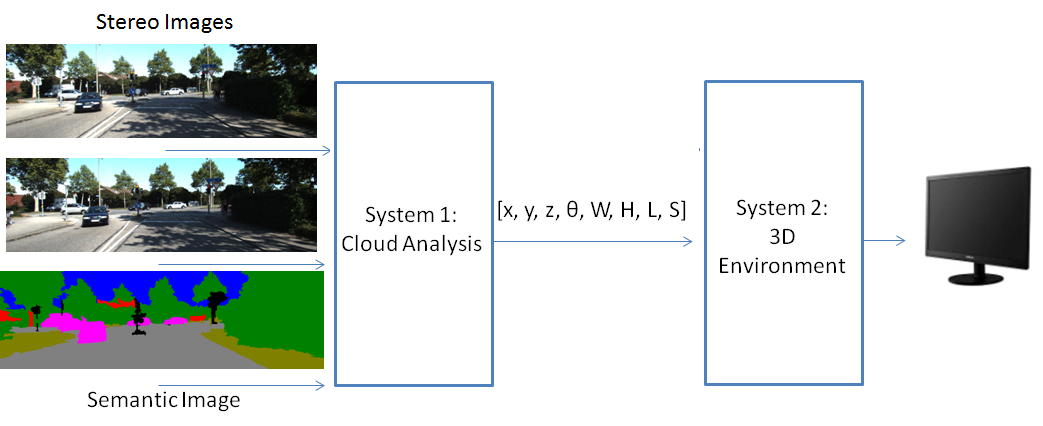
\includegraphics[width=0.85\textwidth]{images/proposed-system-flow-chart.png}
         \end{center}
         \legend{Source: Authors of this study.}
    \end{figure}
    
    The first system named Cloud Analysis is defined by four significant steps: disparity image generation, point cloud creation, semantic association, and feature extraction. It uses concepts of object-oriented programming \cite{object-oriented-modeling-and-design} in its implementation to organize data behavior.
    
    The second system is named 3D environment and has as input information of entities, it represents them in a 3D simulation using computer graphics. The concepts of Entity-Component Systems \cite{house-entity-component-explanation-stack} and Data-Oriented Design \cite{llopis-game-engine-gems-2} are used in its implementation as an approach for better performance results, thus requiring a more in-depth modeling of components and execution flow, which are explored in the development section.

    As contribution, this project delivers an approximation of the environment identified by computer vision algorithms. The system purpose is to bring more confidence to users by offering an interface dedicated to the understanding of algorithms running underneath autonomous vehicles. As future contribution the system can be used for data visualization in case scenarios of surveillance, or accidents by the processing of stored data. 

\section{General Objective}
    
    Elaboration and development of a software for embedded systems to create an estimated representation of the interpretations of Computer Vision algorithms for Autonomous Vehicles.
    
\section{Specific Objectives}

\begin{itemize}
    \item Creating 3D scenes with discriminating categories of objects from generated points clouds using disparity and semantic images;
    \item Describing entities in scenes using feature extraction;
    \item Survey of adequate software architectures and implementations for 3D Environment development;
    \item Development of the 3D Environment visualization software.
\end{itemize}


% ----------------------------------------------------------
% Referencial Teórico
% ----------------------------------------------------------
%!TEX root = TFG.tex

%Definição
%Explicação
%Teoria 
%Ligação com o trabalho

\chapter{Literature Review}\label{literature_review}

\section{State of the Art}

    In this section similar works are cited with the goal of contextualizing our proposal, expressing relations and differences to approaches currently found in the industry and academic research. 

\subsection{Zoox: Simulation for Autonomous Driving}

    Zoox is a startup founded in 2014 with the goal of bringing autonomous mobility experiences to the market. The company is in development stage \cite{zoox-linkedin} and doesn't have widespread marketing campaigns \cite{zoox-official-website}. However, it stands out in the industry due to demonstrations of their autonomous-driving technology. 
    
    The startup made its "tech media" debut on Unreal Engine SIGGRAPH 2017 User Group \cite{zoox-unreal-siggraph-2017} with a technology sneak peek of its simulation pipeline. There they showed a car with 8 sensors as demonstrated in \autoref{fig:zoox-car-sensors} and focused on presenting an elaborate virtual environment with the goal to enhance the passenger experience using visualizations of interpretations of autonomous-driving algorithms as shown in \autoref{fig:zoox-simulation-basic-model}.
    
    \begin{figure}[H]
     \caption{\label{fig:zoox-car-sensors}
Zoox demonstration car}
     \begin{center}
        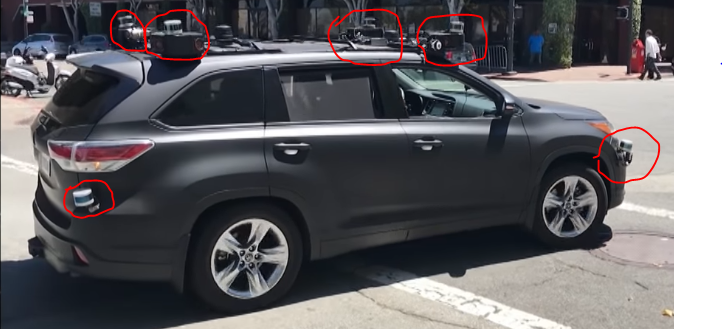
\includegraphics[width=0.8\textwidth]{images/zoox-car_red-lines.PNG}
     \end{center}
     \legend{Source: Adapted from \cite{zoox-unreal-siggraph-2017}.}
    \end{figure}
    
    \begin{figure}[H]
     \caption{\label{fig:zoox-simulation-basic-model}
Zoox simulation environment}
     \begin{center}
        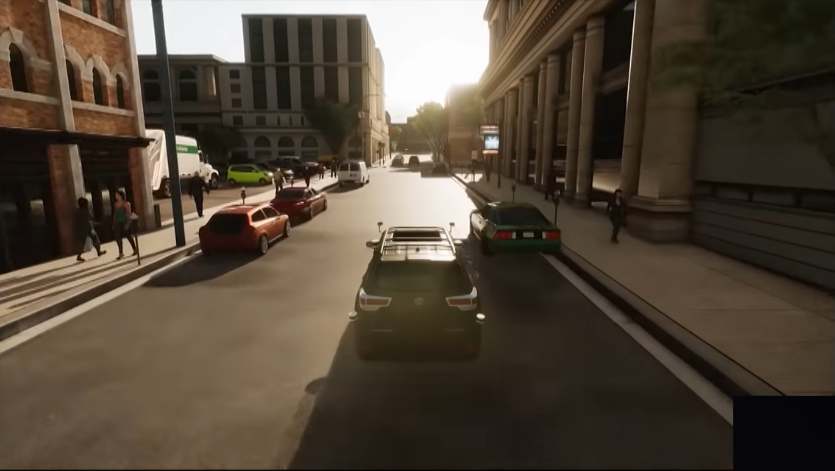
\includegraphics[width=0.8\textwidth]{images/zoox-simulation-basic-model.png}
     \end{center}
     \legend{Source: Adapted from \cite{zoox-unreal-siggraph-2017}.}
    \end{figure}

    On 2018 Zoox introduced their Youtube channel \cite{zoox-youtube-channel} with an evolved demonstration of the route network simulation from SIGGRAPH 2017, shown in \autoref{fig:zoox-siggraph-route-network}, with more entities and an instant route estimation of the autonomous-driving algorithm \cite{zoox-fully-autonomous-driving} as shown in \autoref{fig:zoox-simulation-monitoring}.
    
    \begin{figure}[H]
     \caption{\label{fig:zoox-siggraph-route-network}
Zoox route network}
     \begin{center}
        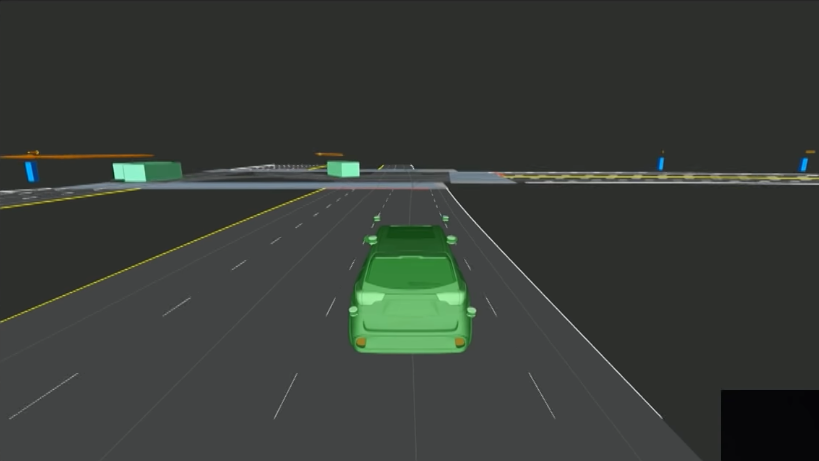
\includegraphics[width=0.8\textwidth]{images/zoox-siggraph-route-network.png}
     \end{center}
     \legend{Source: Adapted from \cite{zoox-unreal-siggraph-2017}.}
    \end{figure}
    
    \begin{figure}[H]
     \caption{\label{fig:zoox-simulation-monitoring}
Zoox simulation environment with route estimation}
     \begin{center}
        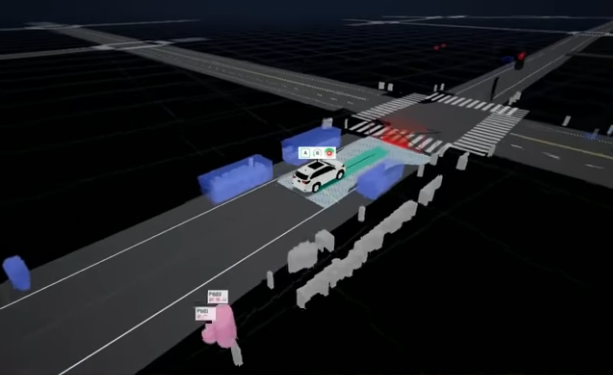
\includegraphics[width=0.8\textwidth]{images/zoox-simulation-monitoring.png}
     \end{center}
     \legend{Source: Adapted from \cite{zoox-fully-autonomous-driving}.}
    \end{figure}
    
    The current work relates to Zoox as both has as goal to provide visualization of autonomous vehicles algorithms. However, the cited startup considers more sensors (Velodyne, LiDAR) than our proposal (two stereo cameras) while also not necessarily focusing on performance for constrained systems.

\subsection{Image Segmentation and Depth}

    One of the major problems in the 3D environment reconstruction and computational vision is to develop a system capable of accurately discriminating each of the elements present in the environment.
    
    For the semantic association problem, \cite{semantic_article} proposes the use of deep convolutional networks in contrast to volumetric approaches operating directly on surface geometry. Crucially, the construction is applicable to unstructured point clouds and other noisy real-world data. The results can be seen in \autoref{fig:semantic-tangent-cnn}.

    \begin{figure}[H]
     \caption{\label{fig:semantic-tangent-cnn}
Top: point cloud from the Semantic3D dataset. Bottom: semantic segmentation produced by the approach.}
     \begin{center}
        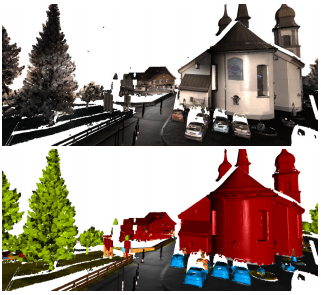
\includegraphics[width=0.5\textwidth]{images/depth_convul.png}
     \end{center}
     \legend{Source: Adapted from \cite{semantic_article}.}
    \end{figure}
    
    The current work relates to \cite{semantic_article} by having point clouds as input. However, while \cite{semantic_article} associate semantic meaning to data, our work have as input semantic images obtained by the current autonomous-driving algorithm in the environment.
    
    Aside from a semantic approach, to accurately discriminate elements in a scene for a virtual representation, it's important to estimate the distance and position of elements. \cite{toyota-depth} is an example of work that tries to improve the state of art on depth estimation (results shown in \autoref{fig:depth-superdepth}).

    \begin{figure}[H]
     \caption{\label{fig:depth-superdepth}Trained Monocular
disparity estimation network in a self-supervised manner
using a synchronized stream of stereo imagery, relieving
the need for ground truth depth labels}
     \begin{center}
        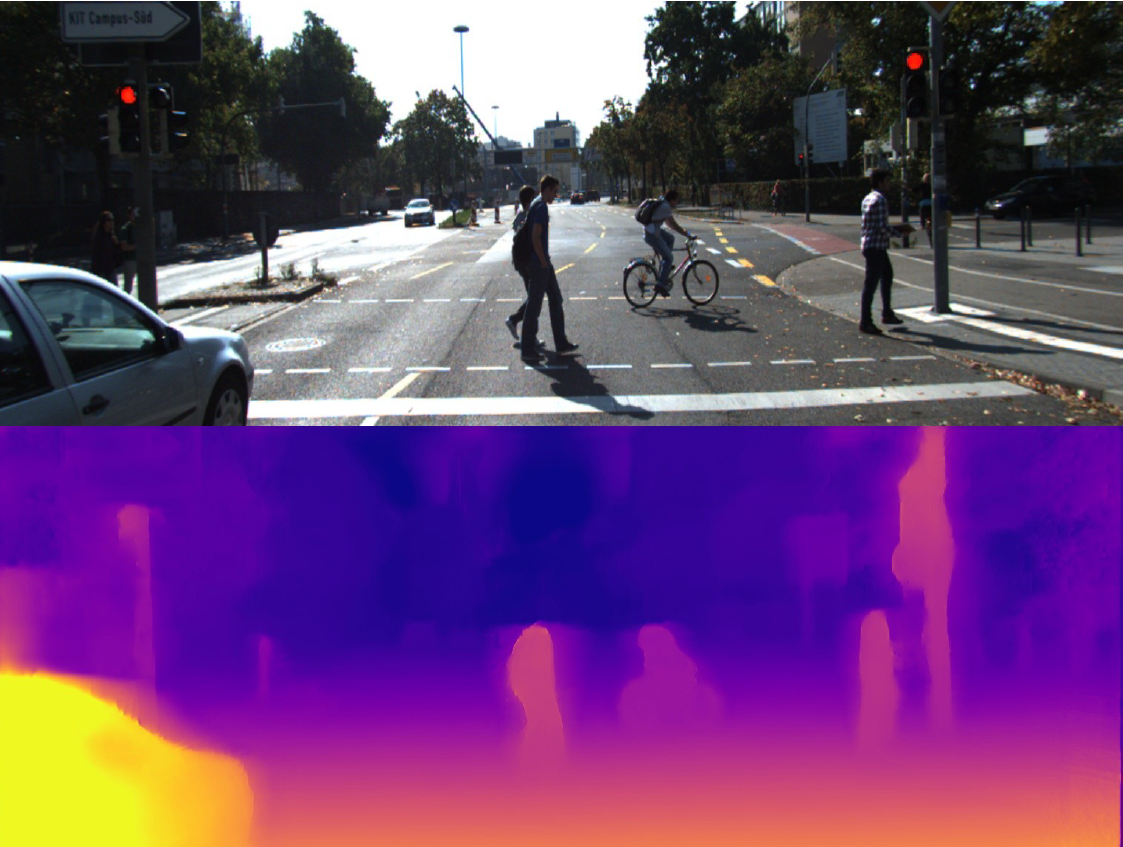
\includegraphics[width=0.45\textwidth]{images/superdepth-toyota.PNG}
     \end{center}
     \legend{Source: \cite{toyota-depth}}
    \end{figure}

    The current work doesn't focus on the creation of a new depth estimation method, as this topic deserves a research of its own. However, on the proposed system depth calculation is part of the pipeline, and a method for it will be explored on the development section.

\subsection{CARLA: An Open Urban Driving Simulation}

    According to CARLA's Website \cite{carla-official-website}, it's a simulator developed from the ground up to support development, training, and validation of autonomous urban driving systems. A open-source project that provides open digital assets (urban layouts, buildings, vehicles) that were created for this purpose and can be used freely. It is a complex simulator platform that supports flexible specification of sensor suites and environmental conditions (such as in \autoref{fig:carla_urban_environment}). In this platform it's possible to test a several kind of system that needs a urban environment. In addition, the system can generate performance reports.
    
    \begin{figure}[H]
     \caption{\label{fig:carla_urban_environment}
A street in Town 2, shown from a third-person view in four weather conditions. Clockwise from top left: clear day, daytime rain, daytime shortly after rain, and clear sunset.}
     \begin{center}
        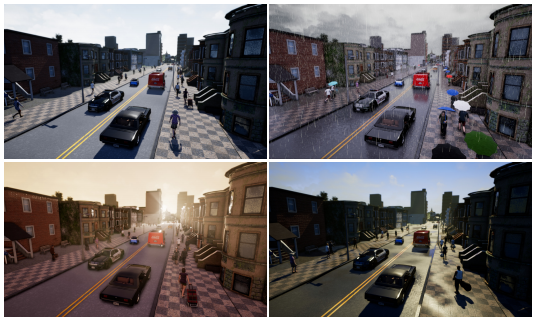
\includegraphics[width=0.8\textwidth]{images/urban_environment.png}
     \end{center}
     \legend{Source: Adapted from \cite{Dosovitskiy17}.}
    \end{figure}
    
    The simulator engine is defined primarily in the paper \cite{Dosovitskiy17} as the development of the environment and sensors. The environment, as shown in \autoref{fig:carla_urban_environment}, is composed of 3D models of static objects such as buildings, vegetation, traffic signs, and infrastructure, as well as dynamic objects such as vehicles and pedestrians. And then the authors used the following steps to build urban environments: (a) laying out roads and sidewalks; (b) manually placing houses, vegetation, terrain, and traffic infrastructure; and (c) specifying locations where dynamic objects can appear (spawn).
    
    About the sensors, CARLA allows for flexible configuration of the agent’s sensor suite. At the time of writing, sensors are limited to RGB cameras and to pseudo-sensors that provide ground-truth depth and semantic segmentation, such as \autoref{fig:carla_sensors}.
    
     \begin{figure}[H]
     \caption{\label{fig:carla_sensors}
Three of the sensing modalities provided by CARLA. From left to right: normal vision camera, ground-truth depth, and ground-truth semantic segmentation. Depth and semantic segmentation are pseudo-sensors that support experiments that control for the role of perception. Additional sensor models can be plugged in via the API.}
     \begin{center}
        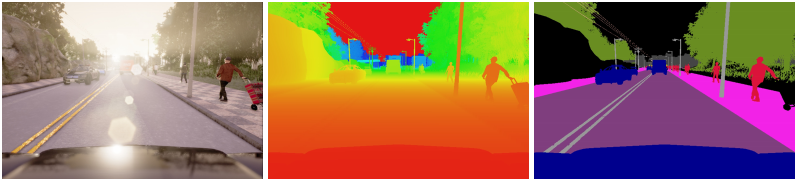
\includegraphics[width=0.8\textwidth]{images/sensor_carla.png}
     \end{center}
     \legend{Source: Adapted from \cite{Dosovitskiy17}.}
    \end{figure} 

    The sensors are be able to segmented 12 semantic classes: road, lane-marking, traffic sign, sidewalk, fence, pole, wall, building, vegetation, vehicle, pedestrian, and other. Therefore, CARLA manages not only to create a realist urban environment, but also to provide tools that allow the complete analysis of the environment around the car.
    
    The current work relates to CARLA as both proposes software with the use of computer graphics to assist the field of autonomous driving. However, CARLA's provides a virtual environment to test autonomous driving algorithms and compare them, while this research is focused in representing an approximation of the environment surrounding a real autonomous car and considering constraints of the real-world (as intrinsic sensor noise and computational limitation).

\section{Point Cloud Generation}

    This section contains concepts utilized to generate point cloud of a scene, and from it extract entity information by feature extraction methods. Point clouds generation steps are separated as camera calibration; disparity and semantic images generation and point cloud creation. These steps can be conceptual defined as the \autoref{fig:conceptual_flow} shows. 
    
        \begin{figure}[H]
     \caption{\label{fig:conceptual_flow}
Conceptual Flow to Generate a Point Cloud}
     \begin{center}
        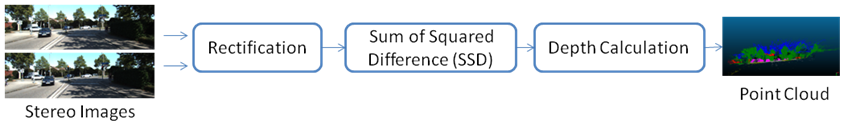
\includegraphics[width=1\textwidth]{images/conceitual_flow.png}
     \end{center}
     \legend{Source: Authors of this study.}
    \end{figure}
    
    As in \autoref{fig:conceptual_flow} flow, one must first calibrate the system according to the camera configuration used by conducting image rectification. Next, the Sum of Square Difference (SSD) calculation is used to obtain the disparity map and then calculate the depth of each scene element. The following subsections explain each of these steps in detail.
    
\subsection{Camera Calibration}

    Cameras have a natural distortion due to physics constraints and different types of lens. The more common are the Barrel and Pincushion distortions, and, according to \cite[p.1]{Vass2003ApplyingAR} “The first is due to the fact that many wide angle lenses have higher magnification in the image center than at the periphery. This causes the image edges to shrink around the center and form a shape of a barrel”. On the other hand, the Pincushion has the opposite effect, causing many wide angle lenses to have high magnification in the periphery of the image. Both are shown in \autoref{fig:lens-distortion}. It’s important to calibrate the cameras in order to eliminate these distortions as much as possible. 
    
    \begin{figure}[H]
     \caption{\label{fig:lens-distortion}
Types of radial distortion (a) Ideal image with no distortion, (b) Barrel Distortion, (c) Pincushion Distortion.}
     \begin{center}
        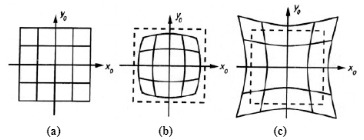
\includegraphics[width=0.7\textwidth]{images/lens.png}
     \end{center}
     \legend{Source: \cite{lensRef}.}
    \end{figure}    
    
    In addition to distortion, calibration is also important for obtaining intrinsic parameters. According to \cite{cameraCalibration1}, "the intrinsic parameters serve to relate the pixel coordinates relative to the images with the coordinates of points of space measured in the referential system originating in the center of the chamber. These parameters depend exclusively on the physical characteristics of the camera (its internal geometry, lens type) ". \cite{cameraCalibration2}, in a laboratory report, shows the main intrinsic parameters to be observed: Focal Distance, Optical Center of the image, Coefficient of lag, and, of course, distortions.

    The focal length, in pixels, represents the distance between the projection center and the image plane; The optical center represents the coordinates of the optical center of the image in frame memory; The lag coefficient represents the angle between the x-axis, y-axis, z-axis of the image in frame memory and the distortions representing the radial and tangential distortion coefficients.
    
    This research uses the distortions parameters, camera matrix and dataset with street pictures publicly available \cite{Geiger2013IJRR}.

\subsection{Epipolar Geometry}

    Epipolar Geometry refers to a mathematical operation that indicates how far apart the components of a scene are. With the help of two cameras (stereo cameras) it is possible to cross similar points of the same image and trace their spatial differences.

    To understand the concept of epipolar geometry, it is necessary to understand the line of projection. Considering an image of any scene, as shown in \autoref{fig:epipolar00}, it can be said that the projection line is the black line that cuts perpendicularly the image. In addition, for understanding, it is necessary to consider \(O_{1}\) the plane that the camera is and \(U_{1}\) the plane that shows the scene of the image.
    
    \begin{figure}[H]
     \caption{\label{fig:epipolar00}
Projection Line}
     \begin{center}
        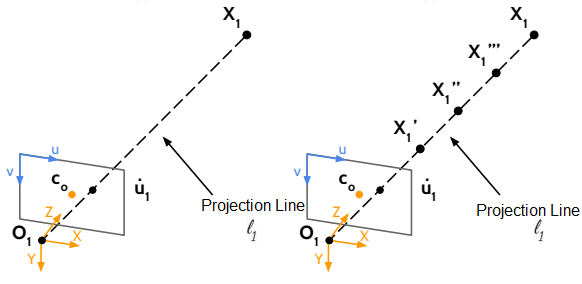
\includegraphics[width=0.5\textwidth]{images/epipolar0.png}
     \end{center}
     \legend{Source: Adapted from \cite{geometriaEpipolarLeonardo}.}
    \end{figure}

    It can be noted by looking at the image that any object located above the projection line (represented by \(X^{'}\), \(X^{''}\) and \(X^{'''}\)) will be superimposed (or hidden). The disparity matrix serves precisely to understand, from images, the depth of this projection line. And for this, a second camera is used, as shown in \autoref{fig:epipolar01}.

    \begin{figure}[H]
     \caption{\label{fig:epipolar01}
Triangulation of a point}
     \begin{center}
        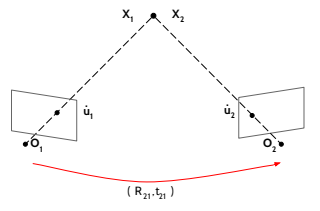
\includegraphics[width=0.5\textwidth]{images/epipolar1.png}
     \end{center}
     \legend{Source: \cite{geometriaEpipolarLeonardo}.}
    \end{figure}
    
    It is possible to see the projection line using a second camera. Therefore it's also possible to match common points between these images, such as in \autoref{fig:epipolar02}.

    \begin{figure}[H]
     \caption{\label{fig:epipolar02}
Matching Points}
     \begin{center}
        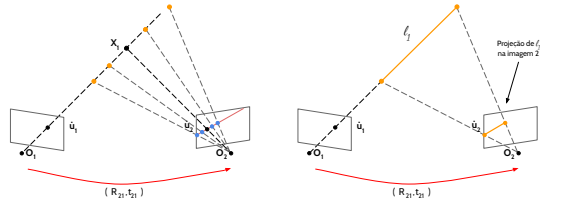
\includegraphics[width=0.7\textwidth]{images/epipolar2.png}
     \end{center}
     \legend{Source: \cite{geometriaEpipolarLeonardo}.}
    \end{figure}
    
    By treating the two images, eliminating their distortions and rectifying one against the other, it is possible to obtain something called the "Baseline" \cite{geometriaEpipolarLeonardo}, shown in \autoref{fig:epipolar03}.

    \begin{figure}[H]
     \caption{\label{fig:epipolar03}
Baseline}
     \begin{center}
        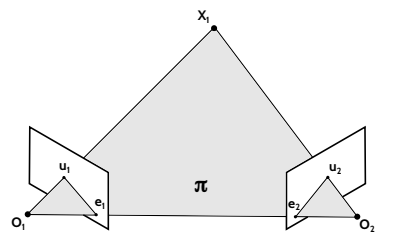
\includegraphics[width=0.5\textwidth]{images/epipolar3.png}
     \end{center}
     \legend{Source: \cite{geometriaEpipolarLeonardo}.}
    \end{figure}
    
    In his thesis \cite{geometriaEpipolarLeonardo} explain that with this configuration it's possible to define a \(\pi\) plane.
    
    The point \(e_{1}\), called the epipolo, is a projection of the optical center of the camera 2 (\(O_{2}\)) in the plane of the image of the camera 1. The epipolo \(e_{2}\) is found in the same way. The line is formed by points \(O_{1}\) and \(O_{2}\), where it connects the optical centers of the cameras is called the baseline. Its intersection with the planes of the images form epipolar lines. 
    
\subsection{Disparity and Sum of Squared Difference}

    Disparity matrix is a set containing the x-axis distance differences from two pixels obtained from left and right images. This matrix can be acquired from the pixels similarity (such as \autoref{fig:similaridade}) and Sum of Squared Difference (SSD) calculation, in code it can be obtained by a class called StereoSGBM using the OpenCV framework \cite{openCVCalibration}. This class match the analyzed function from two inputs: the left and right rectified pictures of the same scene, with requirement of having the images in grayscale.
    
    \begin{figure}[H]
     \caption{\label{fig:similaridade}
Camera Stereo configuration and Similarity of pixel}
     \begin{center}
        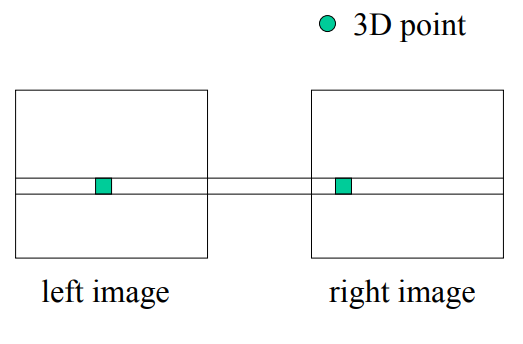
\includegraphics[width=0.5\textwidth]{images/similaridade.png}
     \end{center}
     \legend{Source: \cite{SSD_teste}.}
    \end{figure}
    
    According to the \autoref{fig:similaridade}, the point matching is performed when a common point is found in the two images and the SSD calculation is responsible to find this common pixel. This calculation can be defined by the following equation:
    
    \begin{center}
        \begin{equation}\label{eq:disparidade}
        C_{r}(x, y, d) = \sum_{(u,v)\epsilon W_{m}(x,y)}[I_{l}(u,v)-I_{r}(u-d, v)]^{2}
        \end{equation}
    \end{center}
    
    From the moment images are rectified, it can be stated that: given a horizontal pixel row in an image, there will be a corresponding pixel row in the other image. The SSD calculation is responsible for analyzing pixels in a row and finding the most similar pixels between them. An approach to find the similarity between one pixel and another is to power of two the subtraction of these two pixels, as \autoref{eq:disparidade} shows. Where \(I_{l}\) is the left image; \(I_{r}\) is the right image; \(u\) and \(v\) pixel position coordinates; and \(d\) the variation in \(x\) of the pixel. \autoref{fig:epipolar04} exemplifies the calculation in a more visual manner.
    
    \begin{figure}[H]
     \caption{\label{fig:epipolar04}
SSD Calculation}
     \begin{center}
        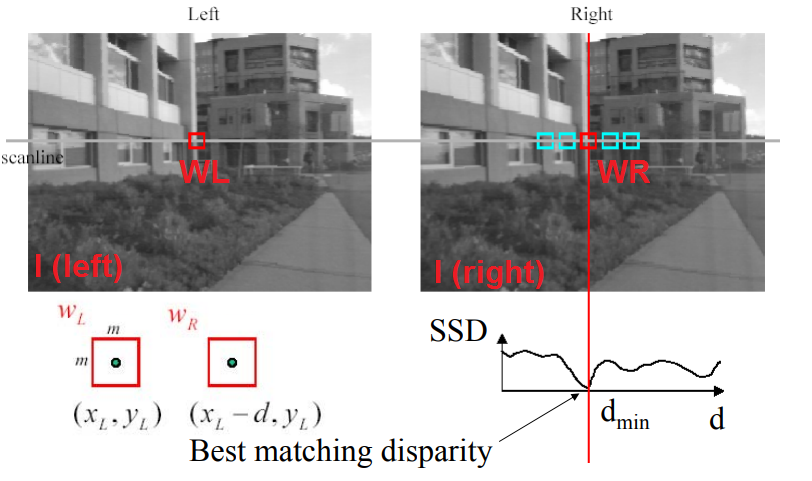
\includegraphics[width=0.9\textwidth]{images/matching_point.png}
     \end{center}
     \legend{Source: \cite{SSD_teste}.}
    \end{figure}
    
    The analysis is faithfully represented by \autoref{fig:epipolar04}, it is possible to observe how each step is performed: First, it defines which pixel should be analyzed in the first image; Next, the pixel row of the second image is defined as the first; Then, the SSD is calculated in the first pixel and its horizontal component varies in order to perform the same subtraction throughout the line; Lastly, it will have a vector of values that will represent which close each pixel of that line is in relation to the the first image pixel. The one with the lowest value will be the pixel most likely to match.
    
\subsection{Point Cloud}

    Point Cloud is a 3D reconstruction of a stereo photo, generated from a disparity map. The function used to do this on the OpenCV framework is called reprojectImageTo3D() and has an important output: A matrix containing x, y and z values with an intensity value in gray scale that shows the distance of each pixel (point) - The closer the camera is to the point, darker is the pixel.
    
    The reprojectImage3D function is an OpenCV feature used to become transparent the calculations and concepts used in the 3D scenario reconstruction. A calculation that uses as epipolar geometry principle and works two important concepts: disparity and depth. Using this geometry, the 3D problem become a 2D problem and thus, it's possible discuss about the disparity and depth concepts. \autoref{fig:epipolar05} evidence how these concepts are joined together for the reconstruction of a 3D scenario.

    \begin{figure}[H]
     \caption{\label{fig:epipolar05}
Disparity and Depth}
     \begin{center}
        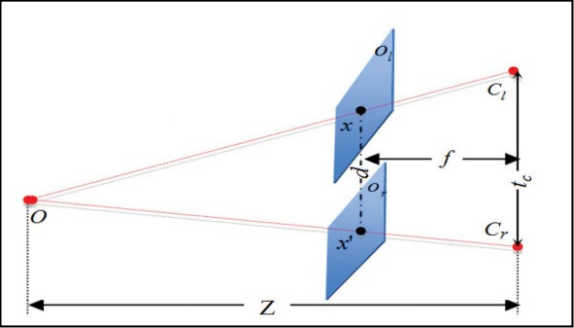
\includegraphics[width=0.8\textwidth]{images/mapaDisparidade.png}
     \end{center}
     \legend{Source: \cite{epipolarDispNat}.}
    \end{figure}
    
    In the image processing conception, it has as disparity the proximity of the same object described in the two images and it has as depth the actual distance of the object in relation to the two cameras.
    
    Similar to \autoref{fig:epipolar03}, it can be stated that once a baseline is defined, the 3D problem around the depth of the elements in the scene becomes two-dimensional similar triangles. Therefore, it can be said that the height of this triangle can be represented by \autoref{eq:profundidade}, since the base of the smaller triangle can be described by the disparity equation, as shown in \autoref{eq:disparidade}.    
    
    \begin{equation}\label{eq:profundidade}
    Z = \frac{t_{c}.f}{d}
    \end{equation}
    \begin{equation}\label{eq:disparidade}
    d = |x_{l}-x_{r}|
    \end{equation}

    Thus, it's possible to discover how deep is each pixel and print them in a 3D scenario. This scenario is called a point cloud.

    There are many applications with a point cloud in a 3D environment. It is usually used in conjunction with an algorithm to treat the surface of these points and reconstruct an approximate image from those points with graphic details. Thus, it's possible to reconstruct the real environment by a 3D environment with details. In the other hand, the point cloud can be used to acquire some useful data without a biggest graphic details, such as: size of different objects in scene, the center of mass, object directions and others.

    The \autoref{fig:point_cloud_ex} shows the point cloud and the possible applications with it. 
    
    \begin{figure}[H]
     \caption{\label{fig:point_cloud_ex}
Point cloud examples}
     \begin{center}
        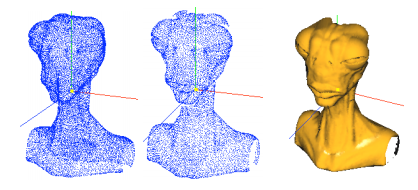
\includegraphics[width=0.8\textwidth]{images/imagem_point_cloud.png}
     \end{center}
     \legend{Source: \cite{pointCloud_ex}.}
    \end{figure}

In the first image, it can be noticed the pure point cloud – a 3D representation of a Alien with points. Alexandre, in his article \cite{pointCloud_ex}, used a reflection conception to describe the image graphically. In the other hand, it’s possible to discover information such as center of mass and substitute the point cloud to an alien's art.

\subsection{Semantic Context}

    A real image is made up of several objects and elements different from each other. In an urban environment, an image can contain pedestrians, cars, streets, animals, houses, poles and other elements that a human can easily differentiate. However, for an algorithm it is a complex task.

    In his thesis, Giovani \cite{giovaniThesis} describes a code capable of performing this objects differentiation in an urban image and compares the results obtained with other algorithms used in the literature. With its algorithm, it is able to discriminate road, sidewalk, vehicles, buildings, sky, vegetation and void spaces - spaces without discrimination.

    Giovani \cite{giovaniThesis} evidences the result of three approaches developed by him: ProbBoost, HistonBoost and ANN (Such as \autoref{fig:semanticaGi}). To use as a parameter and to train the neural network that will contribute to these approaches, the Ground Truth concept is used - an image that graphically represents the differentiation of the objects in the scene, as shown in \autoref{fig:semantic01}.

    \begin{figure}[H]
     \caption{\label{fig:semanticaGi}
Some results of Giovani's Thesis}
     \begin{center}
        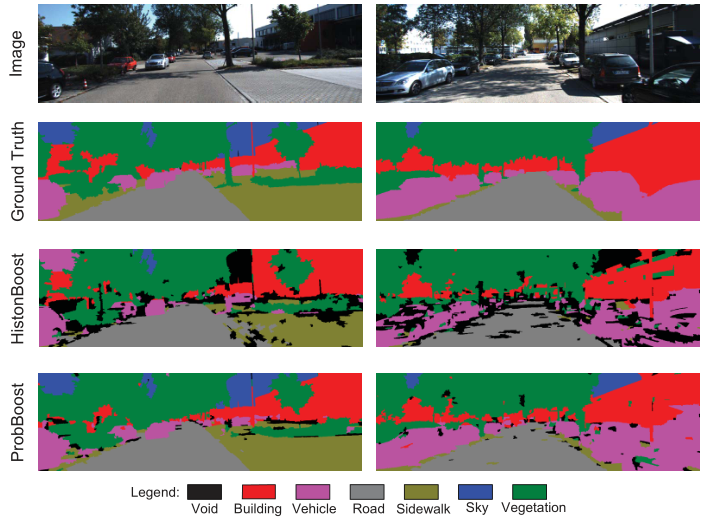
\includegraphics[width=1\textwidth]{images/semanticaGi.png}
     \end{center}
     \legend{Source: \cite{giovaniThesis}.}
    \end{figure}    

    \begin{figure}[H]
     \caption{\label{fig:semantic01}
Semantic Image}
     \begin{center}
        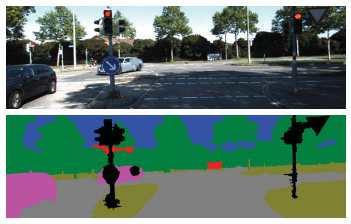
\includegraphics[width=0.7\textwidth]{images/semantic01.png}
     \end{center}
     \legend{Source: \cite{giovaniThesis}.}
    \end{figure}    
    
    In this project, the images generated in the Giovani's research \cite{giovaniThesis} named as Ground Truth are used as a semantic image. The urban environment images are analyzed with the help of the dataset provided by KITTI. KITTI's dataset is an urban image dataset created by Karlsruhe Institute of Technology (KIT).

\subsection{Difficulties}

    \cite{SSD_teste} in his lecture explain that this stereo reconstruction pipeline has some problems. Such as:
    
    \begin{itemize}
    \item Camera calibration errors;
    \item Poor image resolution;
    \item Occlusions;
    \item Violations of brightness constancy (specular reflections)
    \item  Large motions;
    \item Low-contrast image regions;
\end{itemize}

    All of these points are used for the analysis of results.
    
\section{Feature Extraction}

    This section approaches feature extraction methods for appliance on set of points with the final goal of describing entities on a scene. Since this project consider scene semantic information as input. Thus, there is exploration on methods for recognition of different categories. 
    
\subsection{Center of Mass}

    According to \cite[p. 219]{halliday-Mass-Center}, calculating the center of mass of 3D particles is possible by the following equation:
    
    \begin{equation}\label{eq:MassCenterX1}
    x_{mc} = \frac{1}{M}\sum_{i=1}^{n}m_{i}x_{i} 
    \end{equation}
    
    \begin{equation}\label{eq:MassCenterY1}
    y_{mc} = \frac{1}{M}\sum_{i=1}^{n}m_{i}y_{i}
    \end{equation}
    
    \begin{equation}\label{eq:MassCenterZ1}
    z_{mc} = \frac{1}{M}\sum_{i=1}^{n}m_{i}z_{i}
    \end{equation}
    
    Where \(m\) is the weight of the particle and \(M\) is the total weight of all particles together. In the case of a picture, all points have the same weight (value \(1\)) and \(M\) is equal to the total number of particles. Thus, this equation can be simplified to:
    
    \begin{equation}\label{eq:MassCenterX2}
    x_{mc} = \frac{1}{M}\sum_{i=1}^{n}x_{i} 
    \end{equation}
    
    \begin{equation}\label{eq:MassCenterY2}
    y_{mc} = \frac{1}{M}\sum_{i=1}^{n}y_{i}
    \end{equation}
    
    \begin{equation}\label{eq:MassCenterZ2}
    z_{mc} = \frac{1}{M}\sum_{i=1}^{n}z_{i}
    \end{equation}
    
    
\subsection{Box of lower and upper limits of the object}

    There are different ways of calculating limits for a object defined by a set of points. Two approached in this section are the use of center of mass \& geometric centroid, and the analysis tool of variance.

    The first method calculates the center of mass of an object, refer to it as origin, and for each direction calculates the geometric centroid of points, defining them as direction's limit. Repeating this procedure for all directions creates a box which represents the object's approximate size. This approach is not efficient for the reason that it will always set limits lower than the actual limit of the object. Because it is an average of points, this value will hardly match the maximum point of the object.

    On the other hand, \cite{estatistic-douglas} explain a more suitable way of finding these limits. The variance of a random variable is a measure of dispersion, or scatter, in the possible values for the variable. Thus, it's possible to find an approximate value of dispersion for the center of mass (\(\upsilon\)) using the variance formula in \autoref{eq:variance}.

    \begin{equation}\label{eq:variance}
    \sigma^{2} = \sum_{x}(x-\upsilon)^{2}f(x) 
    \end{equation}

    It's possible to find an approximate maximum point of different directions, and then create an upper and lower box of the object, when using \autoref{eq:variance}. Finally, the difference between the upper and lower limits is calculated in order to define the width, height and length values.


\section{3D software architecture}

    This section approaches 3D software architectures considering their motivations, pros \& cons, and implementations. As that one of this project goals is the development of a 3D environment using computer graphics.
    
\subsection{Software Architectures in the industry}

    When considering reference sources for software architectures (especially for 3D and simulation software) the industry related work, e.g. \cite{leonard-thief-postmortem}, stands out as the content theme doesn't appeal strongly to academic environment due to the evident product focused approach instead of theoretical.
    
    Software architecture design choice has direct impact on the performance, as explored in \cite{albrecht-pitfalls-OOP-GCAP09}. Albrecht presented in GCAP 2009 a performance comparison of different data designs implementations. 
    
    The test scene tree consists of an object class containing general data (Object), class to render object (Drawable & Cube), class to update geometrical transforms (Modifier), and container class which store access to objects (Node). The standard data for comparison is shown in \autoref{fig:albrecht-simple-oo-scene-tree}. 
    
    \begin{figure}[H]
        \caption{
        \label{fig:albrecht-simple-oo-scene-tree}
            Simple Scene Tree
        }
        \begin{center}
        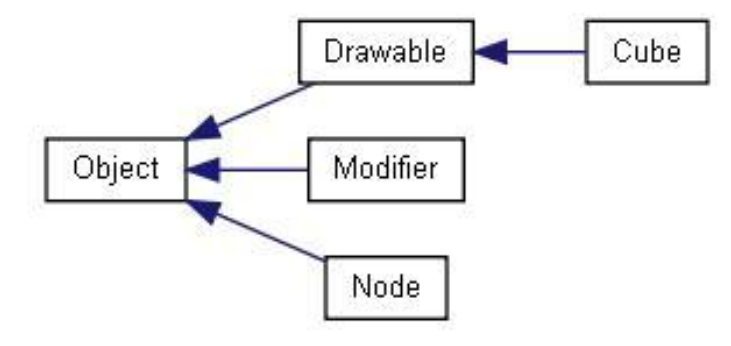
\includegraphics[width=0.5\textwidth]{images/albrecht-simple-oo-scene-tree.png}
        \end{center}
        \legend{Source: Adapted from \cite{albrecht-pitfalls-OOP-GCAP09}.}
    \end{figure}    
    
    The test execution for data in the scene corresponds of:
    
    \begin{itemize}
        \item 11,111 nodes/objects in a tree 5 levels deep
        \item Every node being transformed
        \item Hierarchical culling of tree
        \item Render method being empty
    \end{itemize}
    
    The different data organizations approaches iterate on the previous, and consisting of:
    
    \begin{itemize}
        \item Simple Object Oriented following the Scene tree organization
        \item Contiguous data allocation with use of homogeneous sequential sets
        \item Flat design by removing hierarchy of calls
        \item Flat design with prefetching due to predictable data accesses
    \end{itemize}
    
    Albrecht then presents the final test results for different data designs, shown in \autoref{fig:albrecht-cache-impact}. The most considerable performance gains were obtained by the continuous allocation of data (less encapsulation) and the flattening of hierarchy (less layers of abstraction).  
    
    \begin{figure}[H]
        \caption{
        \label{fig:albrecht-cache-impact}
            Cache impact of different data design approaches (values in milliseconds).
        }
        \begin{center}
        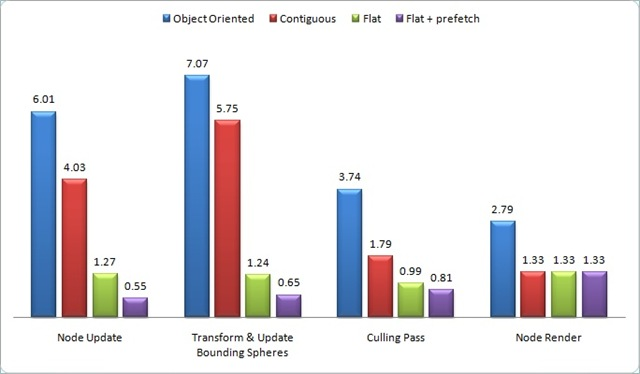
\includegraphics[width=0.8\textwidth]{images/albrecht-cache-impact.jpg}
        \end{center}
        \legend{Source: Adapted from \cite{albrecht-pitfalls-OOP-GCAP09}.}
    \end{figure}
    
    By the previous shown study its evident that to obtain better performance what have to be explored is the way data is accessed and stored. This design approach is justified by the Processor-Memory Gap explored in the next subsection.

\subsection{Processor-Memory Gap}
    
    The Processor-Memory Gap is described by the difference in time between processor memory request and the latency of DRAM access. It describes a problem where the processor performance improved in higher rate than the memory performance improved \cite{computer-architecture-a-quantitative-approach-6ed}. \autoref{fig:performance-gap-processor-memory} shows that the gap increased over many years but is currently in a slowdown due to the lack of improvements in single processors. Although \autoref{fig:performance-gap-processor-memory} shows values for single core processors, the number of multiple cores in processors implies growth of the gap due to the demand of DRAM bandwidth as the number of cores grows.
    
    \begin{figure}[H]
        \caption{
        \label{fig:performance-gap-processor-memory}
            Single processor performance projections against the historical performance improvement in time to access main memory (Processor line shows the increase in memory requests per second on average. Memory line shows the increase in DRAM accesses per second).
        }
        \begin{center}
        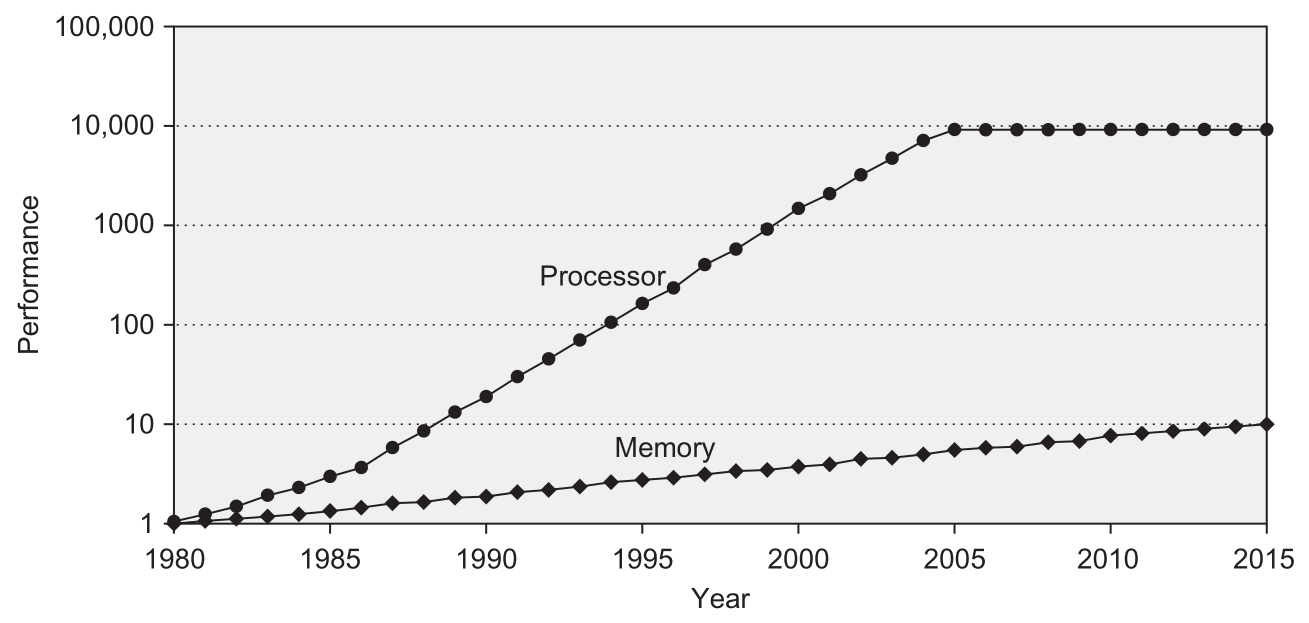
\includegraphics[width=1\textwidth]{images/performance-gap-processor-memory.png}
        \end{center}
        \legend{Source: \cite{computer-architecture-a-quantitative-approach-6ed}.}
    \end{figure}

    As this problem doesn't have an expected hardware solution, it ends up being the software layer job to work with the implied handicap when it appears as an obstacle for an application. In the next subsection we approach Data-Oriented Design, a pattern of software development that is less affect by the Processor-Memory gap problem as the number of memory accesses and cache misses tends to be reduced.
    
\subsection{Entity Component Systems and Data-Oriented Design}

    Entity Component Systems (ECS) is an architectural pattern for software development. There is no concrete definition on its architecture scope, but it does often share Data-Oriented Design (DOD) techniques which focus on designing for performance \cite{llopis-game-engine-gems-2}.
    
    This architecture approach is better suited, for applications such as Game Engines or Real-Time Simulators, which are highly demanding processing software requiring constant main memory access to run in real-time. 
    
    Good case results of implementations for the ECS concept on the industry goes back decades \cite{leonard-thief-postmortem} accompanied by the increased storage of data and the demand of its processing on applications. However, implementation efforts on ECS are still relevant, being focus of features for powerful software \cite{johansson-ecs-unity-gdc-2018}.

    DOD main focus can be considered to be cache coherency. In consequence of this pursue the architecture of code generated by it tends to be decoupled and simple in scope, due to not having a world-approximation as Oriented-Programming encourages. 
    
    As a mean to characterize Data-Oriented Design, \cite{llopis-game-engine-gems-2} consider its benefits and disadvantages. On \autoref{table:dod-benefits} his discourse for each aspect of DOD are listed and simplified.

    \begin{table}[H]
    \centering
    \caption{
        Data oriented design benefits \cite{llopis-game-engine-gems-2}, adaptation as table by Authors of this study.
    }
    \label{table:dod-benefits}
    \begin{tabular}{cc}\toprule
    \textbf{Benefits}                   & \textbf{Description} \\ \bottomrule \\
    Cache utilization                   & \begin{tabular}[c]{@{}l@{}} 
                                        Organization of data into large sequential\\
                                        blocks of homogeneous memory, processing\\ 
                                        it by running the same code on all its\\ elements.\end{tabular}
                                        \\\\ \hline \\
    Parallelization                     & \begin{tabular}[c]{@{}l@{}} 
                                        As we work from the data point of view, it\\ 
                                        becomes a lot easier to divide work up into\\ 
                                        parts that different cores can processes\\ 
                                        simultaneously with minimal synchronization.\\ \end{tabular} \\\\ \hline \\
    Less code                           & \begin{tabular}[c]{@{}l@{}}
                                        Code that before was doing boring book-\\
                                        keeping, or getter/setters on objects,\\ 
                                        or even unnecessary abstractions,\\ 
                                        all go away.\end{tabular}
                                        \\ \\ \bottomrule
    \textbf{Disadvantages}              & \textbf{Description} \\ \bottomrule \\
    It's different                      & \begin{tabular}[c]{@{}l@{}}
                                        So far, data-oriented design isn’t taught\\ 
                                        in Computer Science curricula, \\  
                                        ... so it is foreign to most team members.
                                        \end{tabular} \\\\ \hline \\
    Harder to see the big picture       &  \begin{tabular}[c]{@{}l@{}}
                                        Because of the emphasis on data and on\\
                                        small functions that transform data, it\\
                                        might be harder to see and express the\\
                                        big picture of the program [...]
                                        \end{tabular} \\\\ \bottomrule \\
    \end{tabular}
    \end{table}
    
    A better grasp on the idea of DOD can be obtained with code examples. Consider the two following implementations in C++ \cite{dice-data-oriented-design}. 
    
    \begin{itemize}
        \item \autoref{fig:dice_exampleOOP} uses Object-Oriented Programming and has the idea of creating a class Bot which stores data (attributes) and functionalities (methods);
        \item \autoref{fig:dice_exampleDOP} conforms to the Data-Oriented Design and has as focus generating the output data (in this case the "aiming direction"), doing that with a function which receives the input to be transformed.
    \end{itemize}
     
    \begin{figure}[H]
        \caption{
        \label{fig:dice_exampleOOP}
            Object-Oriented Programming code example
        }
        \begin{center}
        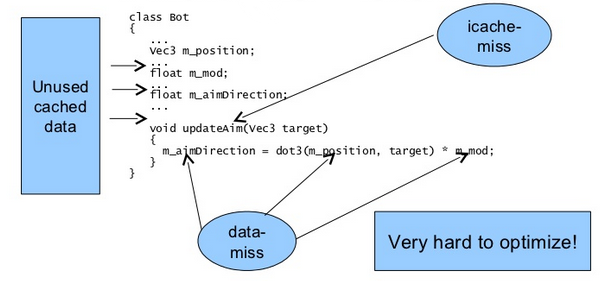
\includegraphics[scale=0.9]{images/dice-exampleOOP_Introduction-to-Data-Oriented-Design.png}
        \end{center}
        \legend{Source: \cite{dice-data-oriented-design}.}
    \end{figure}
    
    \begin{figure}[H]
        \caption{
        \label{fig:dice_exampleDOP}
            Data-Oriented Programming code example
        }
        \begin{center}
        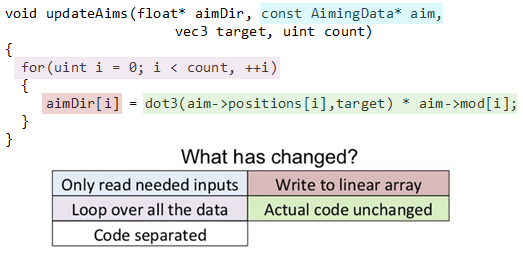
\includegraphics[scale=1]{images/dice-exampleDOP_Introduction-to-Data-Oriented-Design.png}
        \end{center}
        \legend{Source: Adapted from \cite{dice-data-oriented-design}.}
    \end{figure}
    
    It is possible to better visualize the descriptions made in \autoref{table:dod-benefits}, by comparing the two previous implementations. Instead of trying to represent the problem and its elements using known items from the real world as OOP did, DOD focus on solving the problem in its most simpler iteration.
    
    Considering previous data knowledge, as it is likely that there is more than one Bot and that "updateAims" will be called more than once, DOD optimizes memory requests by receiving as parameters the necessary input for processing (aligning it in cache) and doing the same operation for each cell of the "Bots" linear array. Thus eliminating cache misses and decoupling the code.
    
    In conclusion, comparing DOP with the well spread Object-Oriented Programming (OOP), DOP implies the requirement of engineers to know their data, and that structure and code refactoring is continuously present during DOP development to eliminate bottlenecks \cite{albrecht-latency-elephant}.



%%%%%%%%%%%%%%%%%%%%%%%%%%%%%%%%%%%%%%%%%%%%%%%%%%%%%%%%%%%%%%%%%%%%%%%%%%%%%%%%%%%%%%%%%%%%%%%%%%%%%%%%%%%%%%%%%%


% ----------------------------------------------------------
% Projeto Desenvolvido
% ----------------------------------------------------------
 %!TEX root = TFG.tex

\chapter{Development}\label{development}

    The project consists of the development of two isolated systems which interacts with each other. The first system called Cloud Analysis has as input images of a stereo camera and its associated semantic image and as output information of center of mass and objects size in the image - street, house, car, tree, sky, sidewalk and unidentified empty spaces. It was decided to consider only the case scenario with one object of each category of the semantic image in the scene, because it is still not possible to distinguish between two objects of the same category. 

    The second system receives as input the values of the center of mass and size obtained by the first system and then generates a 3D environment of its own with all objects captured by the stereo camera. It uses the Entity Component System approach for its architecture and its implementation is in the C++ language using OpenGL graphics framework.
    
    A representation of the whole system is shown in \autoref{fig:flow-system}, representing both point cloud analysis and 3D environment creation.
    
    \begin{figure}[H]
        \caption{
        \label{fig:flow-system}
            Flow representing the entire system
        }
        \begin{center}
        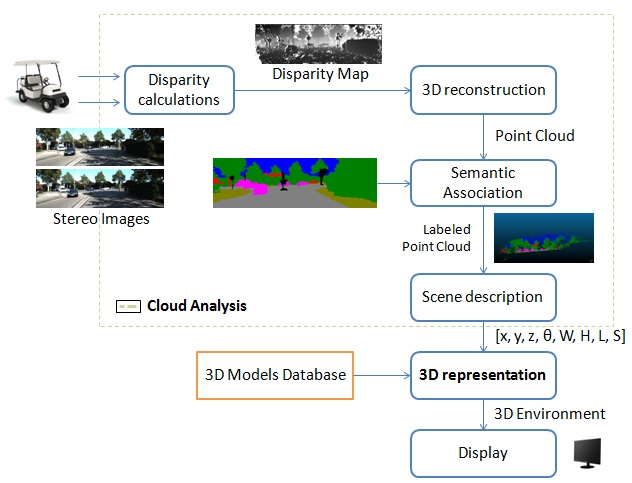
\includegraphics[width=1\textwidth]{images/fluxo1.png}
        \end{center}
        \legend{Source: Authors of this study.}
    \end{figure}    

\section{Cloud Analysis}

    Cloud Analysis is the system capable of generating a number of points which discriminates all categories of the semantic image and calculates their respective center of mass and sizes.
    
    A simple example is to imagine a real urban environment with trees, cars, houses and others. Cloud Analysis has the function of analyzing this scenario and returning the mass center value and size of each of these elements (tree, car and others). It has as output a data tuple of each element, containing: coordinates in the 3D plane of its center of mass, Width, Height, Length and a descriptor that informs which category this element is inserted.

    This system has well-defined steps: disparity image generation, point cloud generation, colored point cloud generation, and center of mass \& size calculation.
    
    For a qualitative analysis, some different tests were performed and each partial flow result can be visualized in the following topics.
    
\subsection{Disparity Calculations}

    The first part of the Cloud Analysis system is the treatment of the two input images for the disparity calculation, as shown in \autoref{fig:disparityCalFlow}. This treatment was performed as follows: The camera calibration data was provided by KITTI dataset and the Sum of Squared Differences(SSD) calculation was used in order to discover the disparity value of each pixel.

    \begin{figure}[H]
        \caption{
        \label{fig:disparityCalFlow}
            Disparity calculation flow}
        \begin{center}
        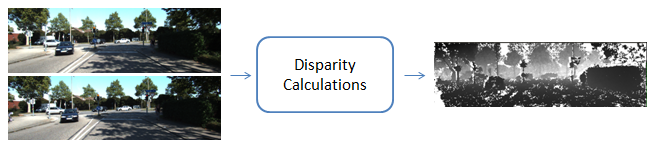
\includegraphics[width=1\textwidth]{images/disparityCalFlow.png}
        \end{center}
        \legend{Source: Authors of this study.}
    \end{figure}
    
    With camera calibration data, it is possible to define the positioning of each of the cameras and to align two images so that the already explained pixel assimilation is possible. The \autoref{Teste1-2results} and \autoref{teste3-4result} show the results obtained in four different scenario tests.

\begin{figure}[H]
  \centering
  \caption{
    The first (left) and second (right) tests and results obtained for disparity image generation. The first three images of each column are inputs (the left and right cameras and the semantic image, respectively \cite{giovaniThesis}). The latter is an image of disparity generated.}
  \label{Teste1-2results}
  \mbox{%
    \subfigure{\label{teste1a}%
      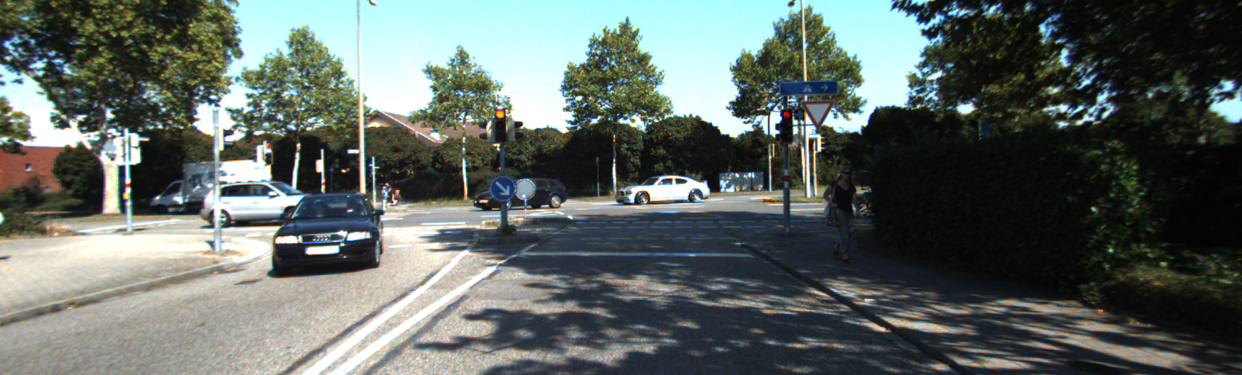
\includegraphics[width=0.4\textwidth]{images/right2.png}}\qquad
    \subfigure{\label{teste2a}%
      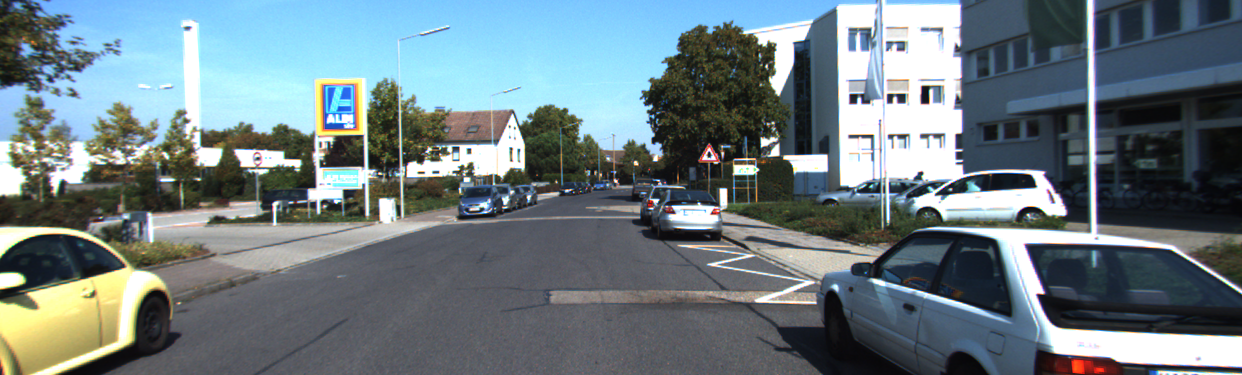
\includegraphics[width=0.4\textwidth]{images/right240.png}}
    }
    \mbox{%
    \subfigure{\label{teste1b}%
      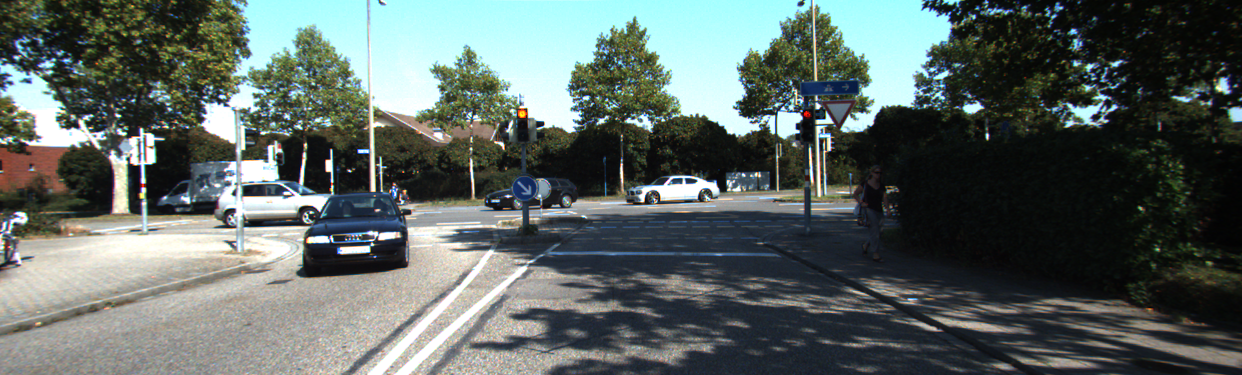
\includegraphics[width=0.4\textwidth]{images/left2.png}}\qquad
    \subfigure{\label{teste2b}%
      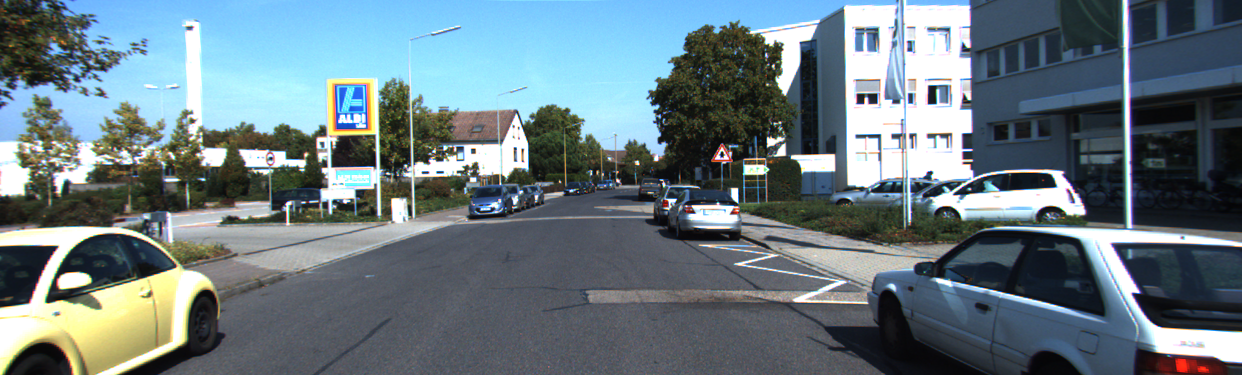
\includegraphics[width=0.4\textwidth]{images/left240.png}}
    }
    \mbox{%
    \subfigure{\label{teste1c}%
      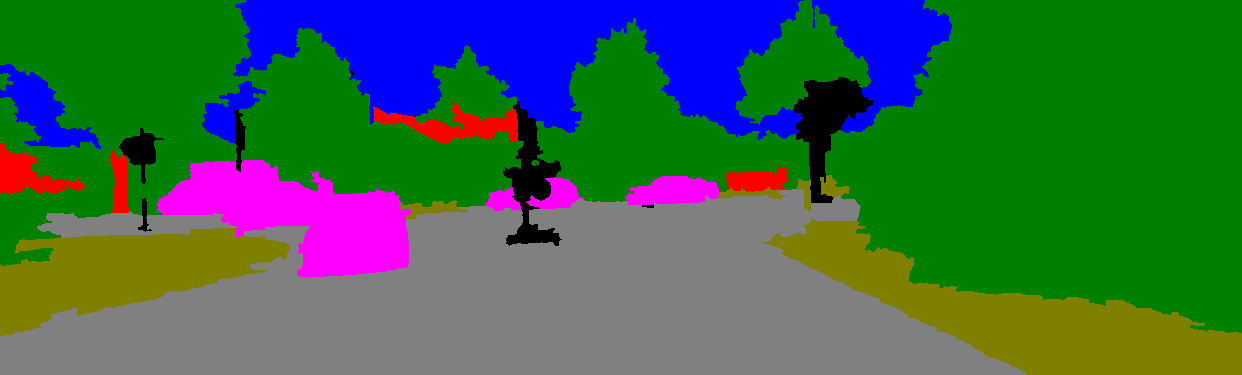
\includegraphics[width=0.4\textwidth]{images/semantica.png}}\qquad
    \subfigure{\label{teste2c}%
      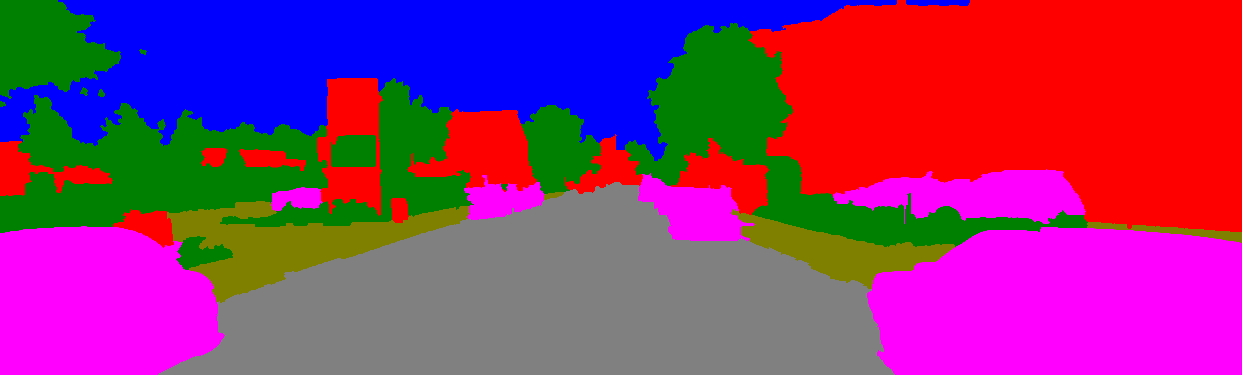
\includegraphics[width=0.4\textwidth]{images/sem240.png}}
    }
    \mbox{%
    \subfigure{\label{teste1d}%
      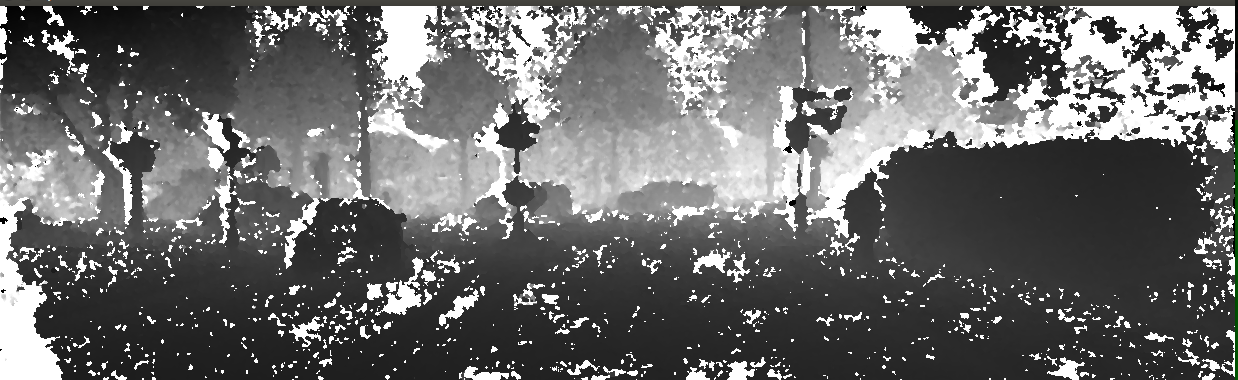
\includegraphics[width=0.4\textwidth]{images/disparity_image.png}}\qquad
    \subfigure{\label{teste2d}%
      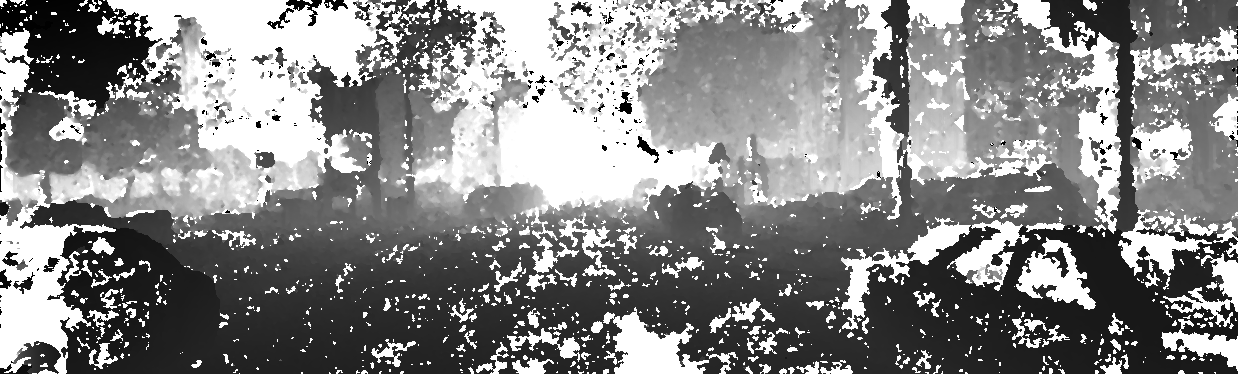
\includegraphics[width=0.4\textwidth]{images/disp240.png}}
    }
    \legend{Source: Authors of this study.}
\end{figure}

\begin{figure}[H]
  \centering
    \caption{
    The third and fourth tests and results obtained for a disparate image generation. The first three images are the system inputs (the left and right cameras and the semantic image, respectively \cite{giovaniThesis}). The latter is an image of disparity generated.
    }
  \mbox{%
    \subfigure{\label{teste3a}%
      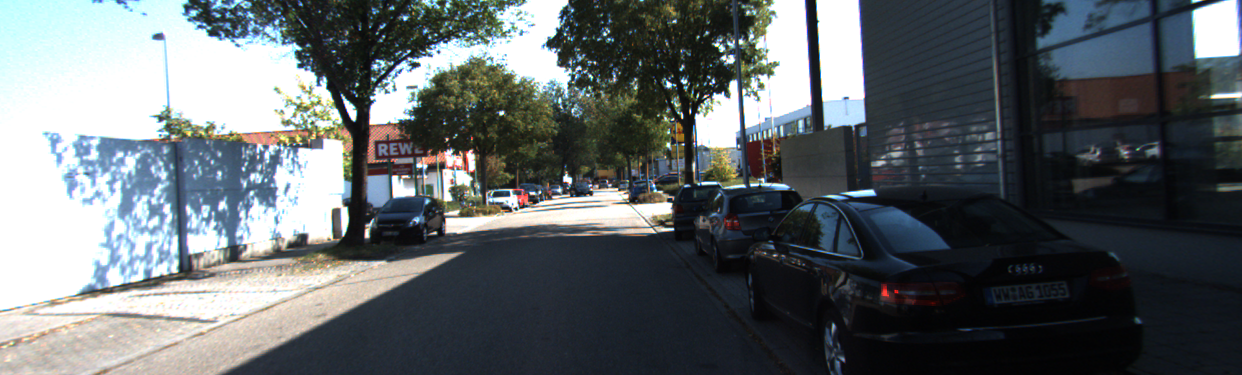
\includegraphics[width=0.4\textwidth]{images/right000.png}}\qquad
    \subfigure{\label{teste4a}%
      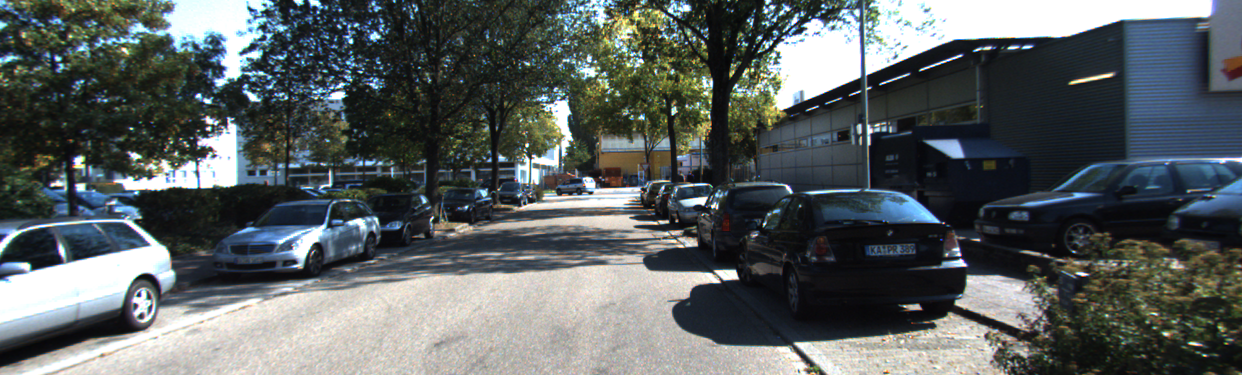
\includegraphics[width=0.4\textwidth]{images/right110.png}}
    }
    \mbox{%
    \subfigure{\label{teste3b}%
      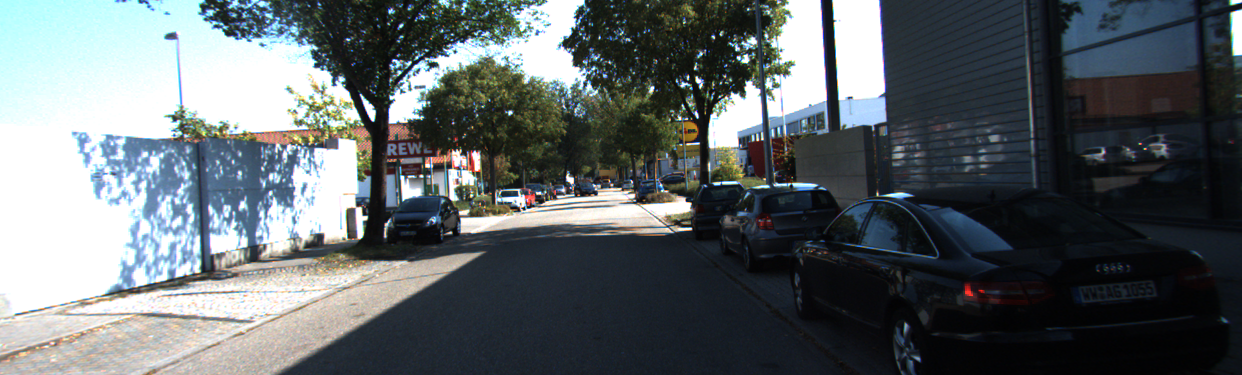
\includegraphics[width=0.4\textwidth]{images/left000.png}}\qquad
    \subfigure{\label{teste4b}%
      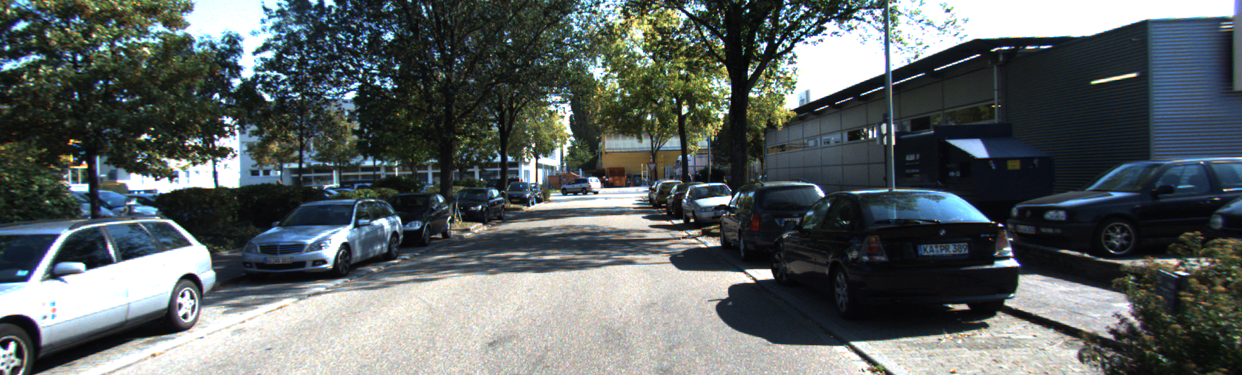
\includegraphics[width=0.4\textwidth]{images/left110.png}}
    }
    \mbox{%
    \subfigure{\label{teste3c}%
      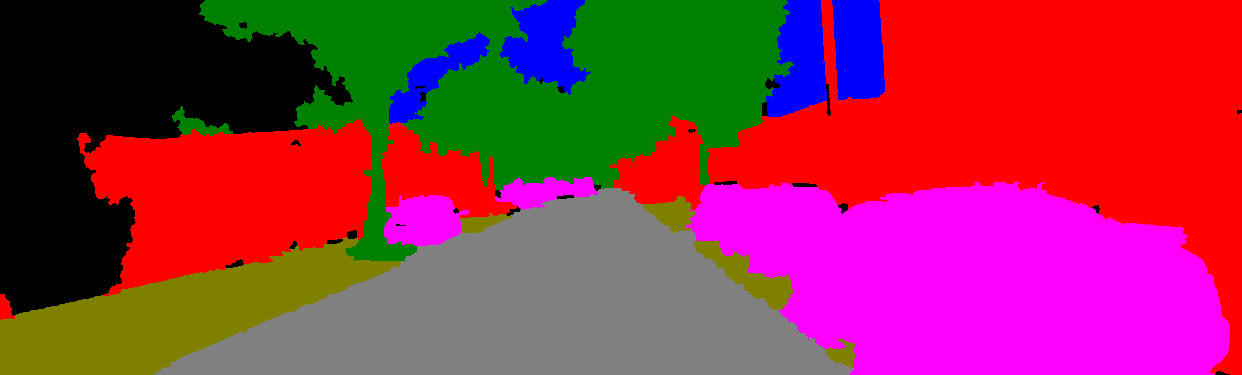
\includegraphics[width=0.4\textwidth]{images/sem000.png}}\qquad
    \subfigure{\label{teste4c}%
      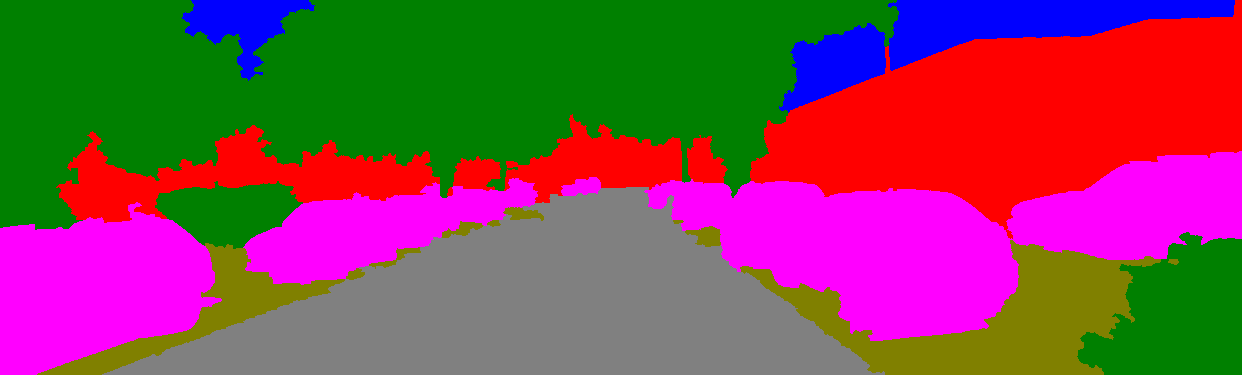
\includegraphics[width=0.4\textwidth]{images/sem110.png}}
    }
    \mbox{%
    \subfigure{\label{teste3d}%
      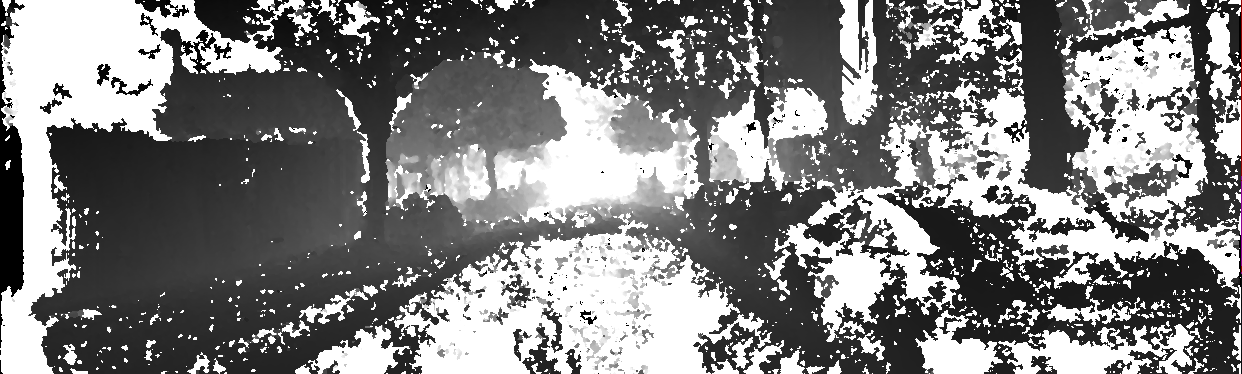
\includegraphics[width=0.4\textwidth]{images/disp000.png}}\qquad
    \subfigure{\label{teste3d}%
      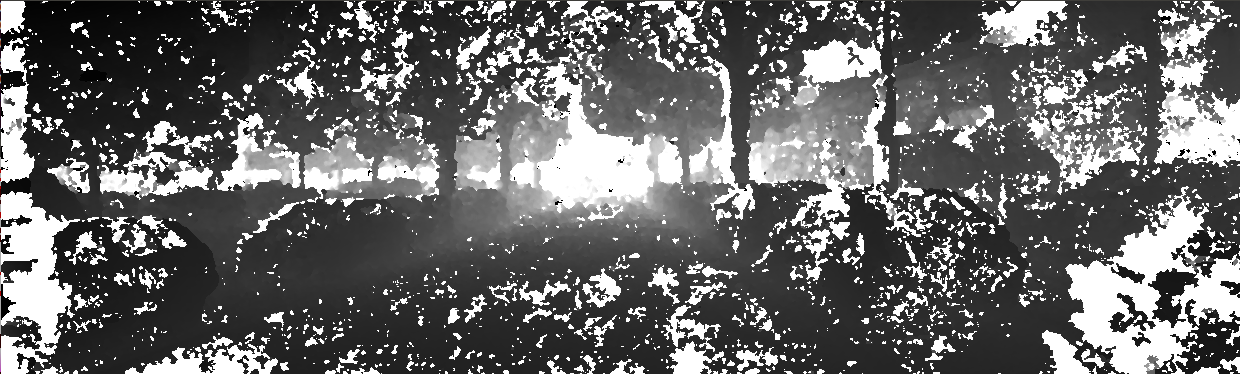
\includegraphics[width=0.4\textwidth]{images/disp110.png}}
    }
    \legend{Source: Authors of this study.}
  \label{teste3-4result}
\end{figure}

    By analyzing the resulting disparity images, one can also perceive that there is a satisfactory proximity to reality. It is possible to perceive the depth of the elements in the images in which the grayscale shows how close or far the components that make up the image are. The third test was shown to be less effective, both in the disparity image and in the color image.
    
\subsection{3D Reconstruction}
    
    The following step in this flow is the point cloud generation, as shown in \autoref{fig:CloudFlow}. 

    \begin{figure}[H]
        \caption{
        \label{fig:CloudFlow}
            Point Cloud Generation Flow}
        \begin{center}
        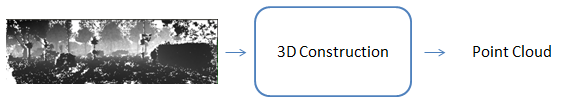
\includegraphics[width=1\textwidth]{images/CloudFlow.png}
        \end{center}
        \legend{Source: Authors of this study.}
    \end{figure}
    
    The Algorithm \autoref{pointCloudAlgo} contains the brief about the whole system developed to create a point cloud. As the Algorithm shows, the result is written in a \textit{xyz} file with 3D points position. In addition to this output, the disparity image was saved so that it could be analyzed.
    
    Using this algorithm, tests were performed using images obtained from Giovani's dataset \cite{giovaniThesis} shown in \autoref{Teste1-2results} and \autoref{teste3-4result} including photos from the right and left camera, and semantic image.

\IncMargin{1em}
\begin{algorithm}
\label{pointCloudAlgo}
\SetKwData{Left}{left}\SetKwData{This}{this}\SetKwData{Up}{up}
\SetKwFunction{Union}{Union}\SetKwFunction{FindCompress}{FindCompres}
\SetKwInOut{Input}{input}\SetKwInOut{Output}{output}
\Input{ Two OpenCV's cv::Mat matrices that represent the right and left photos. In addiction, the respective semantic image of the scene.}
\Output{ A file in \textit{xyz} format that contains a set of 3D points associated to a value. This value represents the distance between the 3D point and the camera.}
\BlankLine
\emph{Camera Calibration according to data collected during camera setup}\;
\emph{Converting photos to grayscale images}\;
\emph{Setup specific values of calibration to use OpenCV's cv::StereoSGBM class}\;
\emph{Disparity image generation by the cv::StereoSGBM class with stereo images as input}\;
\emph{Normalize disparity image to 0-255 scale}\;
\emph{Create a Mat matrix called Points that store 3D points information of the cloud point from the OpenCV's cv::reprojectImageTo3D function}\;    
\For{$i\leftarrow 0$ \KwTo $points.rows$}{
\For{$j\leftarrow 0$ \KwTo $points.cols$}{\label{forins}
\emph{Writing in a \textit{xyz} file the X, Y and Z position of each point and the intensity value (grayscale) related to the distance between point and camera}\;}}
\emph{Printing the result}\;
\caption{Point Cloud Generation}\label{algo_disjdecomp}
\end{algorithm}\DecMargin{1em}

    The image of a point cloud obtained from the photos of left and right is a set of grayscale points with low visualization value as there is to differentiation of entity representation. For this reason, point cloud results were expressed only by the end, in the Colored Point Cloud that uses semantic information to define entities.
    
\subsection{Semantic Association}

    Semantic association means a approach to create a point cloud colored, as shown \autoref{fig:colorFlow}.
    
    \begin{figure}[H]
        \caption{
        \label{fig:colorFlow}
            Semantic Association Flow}
        \begin{center}
        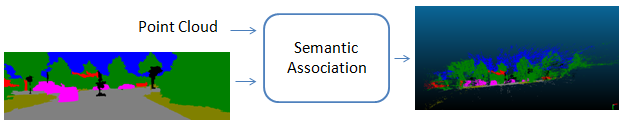
\includegraphics[width=1\textwidth]{images/colorFlow.png}
        \end{center}
        \legend{Source: Authors of this study.}
    \end{figure}
    
    The following steps occurred from the following algorithm: Reading the whole Point Cloud xyz file generated in Algorithm \autoref{pointCloudAlgo}; Reading the semantic image and record the respective RGB (Red, Green and Blue) values to each pixel of the image; Gathering the two values into a single file that contains the following attributes in each row: x, y, and z position of the pixel, its grayscale value and its RGB values.

    There is a program called Cloud Compare that reads \textit{xyz} files and shows the point cloud with color and interact with them. Using this program we were able to display the results shown in \autoref{testeColoredCloud}.

    In \autoref{testeColoredCloud}, each image represents the result of a test, first picture represents first test and the numeration goes top-down. The first test proved to be the most efficient of all which showed a wealth of detail in both near and camera and distant images. The second and fourth tests were also close to reality, especially near the camera.

    The worst test generated was the third test. In this test, the disparity image generated and its point cloud interpreted much of the street as something below the ground, as shown in \autoref{testeColoredCloud} (gray pixels filling the subsoil). It seems that it is related to the fact that the section with few details is very dark, which leads to difficulties in the generation of the disparity image. In addition, it is noted that the semantic image for this photo interpreted as void space much of the sky on the left.
    
\begin{figure}[H]
  \centering
    \caption{
    Colored Point Cloud results}
    \subfigure{\label{testeColor1}%
      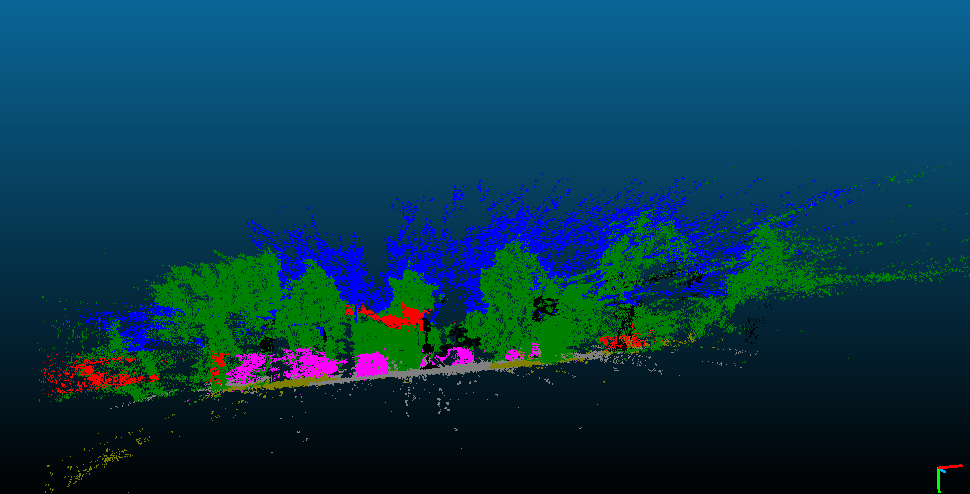
\includegraphics[width=0.6\textwidth]{images/color2.png}}\qquad
    \subfigure{\label{testeColor2}%
      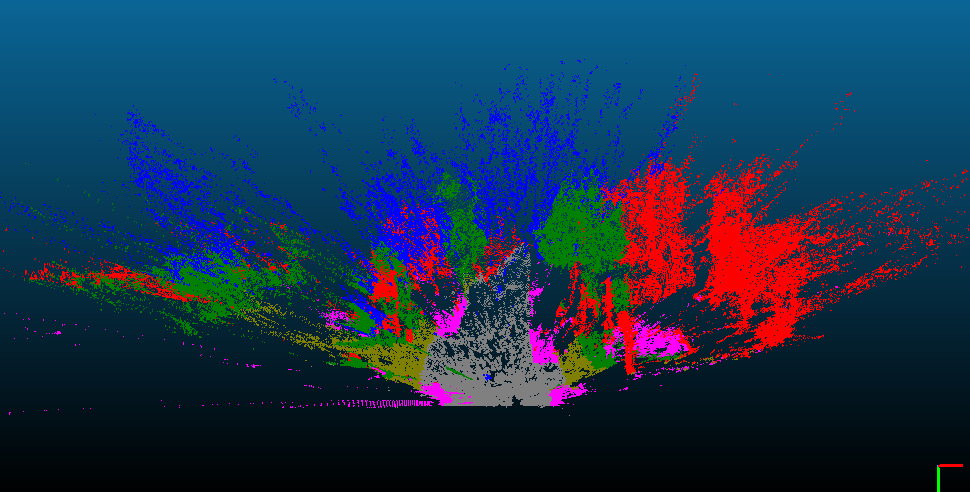
\includegraphics[width=0.6\textwidth]{images/color240(2).png}}\qquad
    \subfigure{\label{testeColor3}%
      \includegraphics[width=0.6\textwidth]{images/color000(2).png}}\qquad
    \subfigure{\label{testeColor4}%
      \includegraphics[width=0.6\textwidth]{images/color110(2).png}}
    \legend{Source: Authors of this study.}
  \label{testeColoredCloud}
\end{figure}    

    
\subsection{Scene Description}

    After the 3D coordinate data and colors have been acquired in the algorithm to obtain the colored point cloud, it is necessary to discriminate the categories and calculate the center of mass and size of each one of them. The flow to do this is represented in \autoref{fig:SceneFlow}. Note that x, y and z represent the x, y, and z coordinates of the center of mass; Theta is the direction of the object in the 3D scenario; W, H and L are the width, height and length that will define the space that the object occupies and S represents what kind of object it is (such as house, vehicle, street and others).
    
    \begin{figure}[H]
        \caption{
        \label{fig:SceneFlow}
            Scene Description Flow}
        \begin{center}
        \includegraphics[width=1\textwidth]{images/sceneFlow.png}
        \end{center}
        \legend{Source: Authors of this study.}
    \end{figure}    
    
    The project is still not able to discriminate a car from another car in the same scene, or a tree from another. Thus, it was decided that the system would assume that there would be only one possible entity: one car, one tree, one building and so on. After the system is able to operate under these conditions it would proceed to a more advanced stage of distinguishing objects within the same category.

    Before calculating the center of mass and the size of the categories contained in the scene, it was necessary to separate them. Thus, an algorithm was developed to read the \textit{xyz} file of the colored point cloud and to separate into a data structure each of the points with equal colors. All the pink objects were stored in a structure called a car, the blues in the structure called sky and the logic remain for the other categories that the semantic image can distinguish.

    Since the assumption is that the system has one element of each category, it is sufficient to calculate the center of mass (\autoref{eq:MassCenterX2}, \autoref{eq:MassCenterY2}, \autoref{eq:MassCenterZ2} ) of each structure separately. In the end, there are seven different center of mass values: One for car, building, tree, sky, sidewalk, street and unidentified void space.

    At this moment, only the calculation of the average of points located in the different directions in relation to the center of mass is done, forming a type of box that would delimit the object boundaries.
    
    To validate the center of mass values, some tests were performed where there is only one element of a certain category in the image. This element had its center of mass calculated and printed on Point Cloud Colored. The first test performed can be seen in \autoref{Teste1Center}. These are two different images in which there is only one car - one car in the first column and one car behind a sign in the second column. In this test it can notice the entire development flow of Cloud Analysis so far: Receiving three images as input and generating a disparity map, a Point Cloud, and output tuples with the center of mass information and size.

    \begin{figure}[H]
  \centering
  \caption{
First and second tests performed with only one car on the scene}
  \label{Teste1Center}
  \mbox{%
    \subfigure{\label{teste1a}%
      \includegraphics[width=0.4\textwidth]{images/right415.png}}\qquad
    \subfigure{\label{teste2a}%
      \includegraphics[width=0.4\textwidth]{images/right410.png}}
    }
    \mbox{%
    \subfigure{\label{teste1b}%
      \includegraphics[width=0.4\textwidth]{images/left415.png}}\qquad
    \subfigure{\label{teste2b}%
      \includegraphics[width=0.4\textwidth]{images/left410.png}}
    }
    \mbox{%
    \subfigure{\label{teste1c}%
      \includegraphics[width=0.4\textwidth]{images/sem415.png}}\qquad
    \subfigure{\label{teste2c}%
      \includegraphics[width=0.4\textwidth]{images/sem410.png}}
    }
    \mbox{%
    \subfigure{\label{teste1d}%
      \includegraphics[width=0.4\textwidth]{images/disp415.png}}\qquad
    \subfigure{\label{teste2d}%
      \includegraphics[width=0.4\textwidth]{images/disp410.png}}
    }
    \mbox{%
    \subfigure{\label{teste1d}%
      \includegraphics[width=0.4\textwidth]{images/color415.png}}\qquad
    \subfigure{\label{teste2d}%
      \includegraphics[width=0.4\textwidth]{images/color410.png}}
    }
    \mbox{%
    \subfigure{\label{teste1d}%
      \includegraphics[width=0.4\textwidth]{images/zoom415.png}}\qquad
    \subfigure{\label{teste2d}%
      \includegraphics[width=0.4\textwidth]{images/zoom410.png}}
    }
    \legend{Source: Authors of this study.}
\end{figure}
    
    In the last image you can see that the center of mass of the car is also being printed - visually close to what would really be the center of it. On the other hand, the size limits described as small yellow squares around the center of mass were not very efficient. All points are assuming values below the actual size of the vehicle.

    It is also noted in the second column that, although the sign disrupts the complete view of the car, the center of mass values remained faithful.
    
    This test quoted above was calculated from the average points located on each of the six sides around the center of mass, as explained in the Literature Review. In order to improve the obtained results, it was decided to apply the variance method. The result and difference can be seen in \autoref{varianceRes}.

    \begin{figure}[H]
      \centering
        \caption{
        Average method vs Variance method}
        \subfigure{\label{varianceRes}%
          \includegraphics[width=0.6\textwidth]{images/zoom415.png}}\qquad
        \subfigure{\label{testeColor2}%
          \includegraphics[width=0.6\textwidth]{images/var415.png}}\qquad
        \legend{Source: Authors of this study.}
      \label{testeColoredCloud}
    \end{figure} 
    
    It can see that the bounding box is still not perfect. Before it was too small and now, it is bigger than the real. Despite this, both results proved adequate to create a representation of the car's bounding box.It was defined to used the variance.
    
    Another test was performed considering situations where there is only one street. The function of this test is to validate the center of mass calculation of other categories besides vehicles. The street will have a different treatment in the 3D environment, however, the output of Cloud Analysis will be similar to vehicles. As shown in \autoref{Teste2Center}, the street's center of mass is located at a visually expected point, marked orange in the images.
    
    The results obtained from the center of mass (both in \autoref{Teste1Center} and in \autoref{Teste2Center}) are defined in a range of values different from the 3D environment. The functions and calculations performed for the Point Cloud generation return as a result values approximately between 5 and - 5 floating values - which is far from representing a metric close to the metric of reality.
    
    \begin{figure}[H]
  \centering
  \caption{
First and second tests performed with only one street on the scene}
  \label{Teste2Center}
  \mbox{%
    \subfigure{\label{teste1a}%
      \includegraphics[width=0.4\textwidth]{images/right35.png}}\qquad
    \subfigure{\label{teste2a}%
      \includegraphics[width=0.4\textwidth]{images/right310.png}}
    }
    \mbox{%
    \subfigure{\label{teste1b}%
      \includegraphics[width=0.4\textwidth]{images/left35.png}}\qquad
    \subfigure{\label{teste2b}%
      \includegraphics[width=0.4\textwidth]{images/left310.png}}
    }
    \mbox{%
    \subfigure{\label{teste1c}%
      \includegraphics[width=0.4\textwidth]{images/sem35.png}}\qquad
    \subfigure{\label{teste2c}%
      \includegraphics[width=0.4\textwidth]{images/sem310.png}}
    }
    \mbox{%
    \subfigure{\label{teste1d}%
      \includegraphics[width=0.4\textwidth]{images/disp35.png}}\qquad
    \subfigure{\label{teste2d}%
      \includegraphics[width=0.4\textwidth]{images/disp310.png}}
    }
    \mbox{%
    \subfigure{\label{teste1d}%
      \includegraphics[width=0.4\textwidth]{images/color35.png}}\qquad
    \subfigure{\label{teste2d}%
      \includegraphics[width=0.4\textwidth]{images/color310.png}}
    }
    \mbox{%
    \subfigure{\label{teste1d}%
      \includegraphics[width=0.4\textwidth]{images/zoom35.png}}\qquad
    \subfigure{\label{teste2d}%
      \includegraphics[width=0.4\textwidth]{images/zoom310.png}}
    }
    \legend{Source: Authors of this study.}
\end{figure}
    
    In addition, it was noted that the Cartesian plane used follows the pattern shown in \autoref{fig:CartesianPlane}, where the camera located in the car is taken as the axis (0,0,0).

    \begin{figure}[H]
    \caption{
        \label{fig:CartesianPlane}
        Cartesian plane used in Point Cloud
        }
        \begin{center}
        \includegraphics[scale=1]{images/eixos.png}
        \end{center}
        \legend{Source: Authors of this study.}
    \end{figure}
    
    The mass centers of the two cars analyzed in the test of \autoref{Teste1Center} can be seen in \autoref{Table:Center1} while that of the test of \autoref{Teste1Center} can be seen in \autoref{Table:Center2} and them exemplified how lower these numbers are.
    
    \begin{table}[H]
    \centering
    \caption{X, y, and z axis coordinates of the test of \autoref{Teste1Center}}
    %\vspace{0.2cm}
    \label{Table:Center1}
    \begin{tabular}{r|lll}
    Teste & X-axis & Y-axis & Z-axis \\ 
    \hline                               
    Car 1 & -0.417017   & 0.0258149 & 0.628768 \\
    Car 2 & -0.427101   & 0.0166311 & 0.78519       
     
    \end{tabular}
    \end{table}

    \begin{table}[H]
    \centering
    \caption{X, y, and z axis coordinates of the test of \autoref{Teste2Center}}
    %\vspace{0.5cm}
    \label{Table:Center2}
    \begin{tabular}{r|lll}
    Teste & X-axis & Y-axis & Z-axis \\ 
    \hline                              
    Street 1 & -0.193943   & 0.0495407 & 0.698221 \\
    Street 2 & -0.153351   & 0.0435096 & 0.700954   
     
    \end{tabular}
    \end{table}

    Therefore, one has to challenge the construction of a metric to convert these small coordinate values ​​into useful values ​​in the 3D environment
    
\subsection{Errors analysis.}

    This system has well-defined stages for its development and this has the benefit of the facility in identifying errors before are propagated.
    
    The first stage is camera calibration. The calibration itself can carry various types of errors and, according to \cite{ErrosCalibracao}, these can be categorized as:
    
    \begin{itemize}
    \item Gross Errors: This error is caused by the inability or neglect of the measurer;
    \item Accidental (or random) mistakes: These errors are caused by the imperfection of our senses, atmospheric irregularities and inevitable minor errors in instrument construction;
    \item Systematic errors: Errors caused by non-conforming measures (such as dilated timing, bent bolt and dumbbell post);
    \item Rounding Errors: Typically caused by the use of numbers with a few decimal places.

\end{itemize}

    It is possible that the system is subject to all these errors, although there are efforts to avoid them, such as using as many decimals as possible, both in calibration and in subsequent steps.
    
    In the following steps of calculating the disparity map it is possible to highlight some reasons for the difficulties already reported, such as low-contrast image regions. This problem impacted the results shown in order to create holes in the disparity map generating a noise that propagated to the end of the flow and hampered the faithful acquisition of the features.
    
    Another factor that contributed to the difficulty in generating a plausible graphical environment was the fact that the Point Cloud is generated by small coordinates. These values were between 5 and -5, with six decimal places in each coordinate. These low numbers contributed to the propagation of the error, since any small rounding in the center of mass calculation or in the bounding box will already result in very disparate values when passed to the 3D environment.

\section{3D environment}
    
    The 3D environment is expected to receive as input the identified entities, their information (position, direction and size), and standard 3D Model  that better represent it, and as output display an approximate scene from what was identified by the computer vision algorithm. A general flow of expected input and output is shown in \autoref{fig:3D-representation-flow}.
    
    \begin{figure}[H]
    \caption{
        \label{fig:3D-representation-flow}
            3D representation flow
        }
        \begin{center}
        \includegraphics[scale=0.65]{images/3D_representation.png}
        \end{center}
        \legend{Source: Authors of this study.}
    \end{figure}
    
    It was decided to develop the 3D environment system using C++ in conjunction with the graphical framework OpenGL, as it was considered the possibility of resource constraints, such as usage of CPU \& Memory and processing time. The system uses the OpenGL Shading Language (GLSL) for manipulation of VertexShaders and FragmentShaders. These choices, aside from the previous points, were based on authors' affinity with languages and frameworks while also allowing for more control on the program execution and better comprehension of the graphics pipeline of modern frameworks since both options are in a considerable low abstraction layer.
    
\subsection{Software Architecture}
    
    Following the Data-Oriented Design concept presented in the Literature Review chapter, an Entity Component System was projected as shown in \autoref{fig:kagami-simplified-diagram}.
    
    \begin{figure}[H]
        \caption{
        \label{fig:kagami-simplified-diagram}
            3D environment simplified diagram
        }
        \begin{center}
        \includegraphics[scale=0.65]{images/kagami-simplified-diagram.png}
        \end{center}
        \legend{Source: Authors of this study.}
    \end{figure}
    
    The control class of the system can be identified in \autoref{fig:kagami-simplified-diagram} as the class Engine, it has methods to initialize the main loop of the software and contains calls for defined Systems. Aside from the importance of the class Engine, three other classes deserve a more thorough description:
    
    \begin{itemize}
        \item Entity
        
        Represents the objects of the program, it maps the components existent in the software such as objects in a scene.
        
        \item Component
        
        Represents the differentiation of data stored in the program, it is mapped by the Entity class and all it's processing is dependent and executed by System classes. 
        
        \item Systems
        
        Are the real operators of the engine, it runs a defined data transformation (like defined on RendererSystem) on all the correct data of the program in a sequential manner). For example, RendererSystem conducts data transformation of all the entities which contains the Component's inherited class "RenderableComponent".
        
    \end{itemize}

\subsection{Display Evaluation}

    The 3D environment is capable of loading objects with information provided by the Cloud Analysis system. The input is the position coordinates (\(x\), \(y\), \(z\)), its orientation (\(theta\)), its size (Width, Length, Height) and semantic class (Car: 1, Street: 2).

    To evaluate the functionality of the 3D environment, a scene with one car was selected as shown in \autoref{fig:selected_test_visualization}. 
    
    \begin{figure}[H]
          \centering
          \caption{
        Scene for visualization test}
          \label{fig:selected_test_visualization}
            \subfigure{\label{testevisualization1a}%
              \includegraphics[width=0.4\linewidth]{images/right415.png}}\\
            \subfigure{\label{testevisualization1b}%
              \includegraphics[width=0.4\linewidth]{images/left415.png}}\\
            \subfigure{\label{testevisualization1c}%
              \includegraphics[width=0.4\linewidth]{images/sem415.png}}\\
            \subfigure{\label{testevisualization1d}%
              \includegraphics[width=0.4\linewidth]{images/color415.png}}\\
            \subfigure{\label{testevisualization1e}%
              \includegraphics[width=0.4\linewidth]{images/result_pointcloud.png}}\\
            \legend{Source: Authors of this study.}
    \end{figure}
    
    Thus, using \autoref{fig:selected_test_visualization} the point cloud as reference (bottom image), a baseline 3D environment input was crafted using \cite{giovaniThesis} semantic colors as shown in \autoref{fig:crafted_baseline}.
    
    \begin{figure}[H]
          \centering
          \caption{
        Crafted baseline}
          \label{fig:crafted_baseline}
            \subfigure{\label{crafted_baselinea}%
              \includegraphics[width=0.7\linewidth]{images/sem415.png}}\\
            \subfigure{\label{crafted_baselineb}%
              \includegraphics[width=0.7\linewidth]{images/result_pointcloud.png}}\\
            \subfigure{\label{crafted_baselinec}%
              \includegraphics[width=0.7\linewidth]{images/result_tailored.png}}\\
            \legend{Source: Authors of this study.}
    \end{figure}
    
    To evaluate the performance of the first system feature extractors, \autoref{fig:feature_extractors_visualization} shows:
    
    \begin{itemize}
        \item Top-Left: Crafted baseline;
        \item Top-Right: Simplified crafted baseline showing only car and street;
        \item Bottom-Left: Center of mass feature;
        \item Bottom-Right: Variance feature.
    \end{itemize}
    
        \begin{figure}[H]
          \centering
          \caption{
        Feature extractors comparison}
          \label{fig:feature_extractors_visualization}
          \mbox{%
            \subfigure{\label{fig:Ng1}%
              \includegraphics[width=0.5\linewidth]{images/result_tailored.png}}
            \subfigure{\label{fig:Ng2}%
              \includegraphics[width=0.5\linewidth]{images/result_tailored_simplified.png}}
            }
            \mbox{%
            \subfigure{\label{fig:Ng3}%
              \includegraphics[width=0.5\linewidth]{images/result_centerofmass.png}}
            \subfigure{\label{fig:Ng4}%
              \includegraphics[width=0.5\linewidth]{images/result_variance.png}}
            }
            \legend{Source: Authors of this study.}
        \end{figure}
        
    Comparing feature extractors, it's possible to say that the center of mass method showed better results in relation to position but bad due to it's smaller scale in relation to the baseline, while the variance method have better coverage of the baseline car. When considering a user point of view for an interface, the variance method performed better for car representation. 
    
    Since the current Cloud Analysis doesn't provide more than one entity for one semantic class, the street object is on the comparison picture for spatial reference.
    
    Case scenarios are limited due to the constraint of one type of semantic class. However, it's possible to confirm the visualization functionality of the 3D environment.

% ----------------------------------------------------------
% Resultados Obtidos
% ----------------------------------------------------------
\chapter{Conclusion} \label{final_considerations}

%This version goal is to help tailor writing and correct vision mistakes on the project course. It is known by the authors that the content shown here is not perfect, nor is its exposure. But it's intended to collect feedback and suggestions for the final version of this document, such as more recommended literature and different approaches to those presented here and the ones being proposed in the future steps.

%The research is still ongoing. However, it is possible to have conclusions on the progress made. Future steps will also be listed during this chapter.

%\section{Conclusion}\label{conclusao}

It's possible to affirm that an end-to-end version of the proposed system was properly elaborated \& developed, and that the set goals of the research were achieved. However, better results for the visualization were expected when considering that only one semantic class had to exist to enable feature extraction. Thus, limiting the number of test scenarios and variety in the 3D environment representation.

For better performance of the first system, a more elaborate method that could be explored in future work would be to consider clustering entities with the same semantic image information. Thus, still making use of the advantageous semantic information offered by the autonomous-driving algorithm for its decision making, and now considering more than one entity with the same semantic class in a scene. A second point of improvement would be to explore approaches to reduce point cloud noise by using more elaborate depth estimation methods.

To enhance the second system results, future work could involve conducting tests on real embedded systems for autonomous-driving while profiling the software performance, and optimizing it when needed. A parallel approach could involve the building of a display prototype to receive real users feedback and evaluation. 

Finally, an approach on surveillance and monitoring could be explored and evaluated. Possibly considering the use o sensors from more than one vehicle connected by network, and also exploring the possibility of map update following the graphical display procedure achieved in this research.


%\section{Future Work}\label{trabalhos_futuros}


%    With the end of this first stage of development, note some important steps that must be taken in this next research phase. Regarding the first point cloud analysis system, the following points should be worked: Use the variance model to obtain the most efficient object size in the scene; to study ways to generate an approximate plane equivalent to the plane of the street and sidewalk, beside to study ways to deduce the direction of vehicles from the cloud information points we have. Regarding the second system, you must find ways to convert the coordinate format that the environment receives in a format that makes sense in the developed 3D environment. If it is possible, there is also a desire to be able to discriminate different objects within the same category of the semantic image.


% ----------------------------------------------------------
% Finaliza a parte no bookmark do PDF
% para que se inicie o bookmark na raiz
% e adiciona espaço de parte no Sumário
% ----------------------------------------------------------
\phantompart

% ----------------------------------------------------------
% ELEMENTOS PÓS-TEXTUAIS
% ----------------------------------------------------------
\postextual
% ----------------------------------------------------------

% ----------------------------------------------------------
% Referências bibliográficas
% ----------------------------------------------------------
\bibliographystyle{abntexalfenglish}
\bibliography{reference}

%\printbibliography

%\begin{appendix}

\end{appendix}

\end{document}
